\documentclass[oneside,brudnopis]{xelatex-mgr/xmgr}

\usepackage{amsmath}
\usepackage{amssymb}
\usepackage{blindtext}
\usepackage{tikz}
\usepackage{amsthm}
\usepackage{algorithmicx}
\usepackage{algpseudocode}
\usepackage{booktabs}

\usetikzlibrary{calc}
\usetikzlibrary{intersections}
\usetikzlibrary{patterns}
\tikzset{>=latex}

% \defaultfontfeatures{Scale=MatchLowercase}
\setmainfont[Numbers=OldStyle,Mapping=tex-text]{Minion Pro}
\setsansfont[Numbers=OldStyle,Mapping=tex-text]{Myriad Pro}
\setmonofont[Scale=0.75]{Monaco}

\wersja{wersja wstępna [\ymdtoday]}

\author{Bartłomiej Kruczyk}
\nralbumu{213603}
\email{bartlomiej.kruczyk@gmail.com}

\title{Efektywne algorytmy dla wielokątów wypukłych}
\date{2014}
\miejsce{Gdańsk}

\opiekun{dr hab. Paweł Żyliński}

\theoremstyle{definition}

\newtheorem{twierdzenie}{Twierdzenie}[chapter]
\newtheorem{problem}{Problem}[chapter]
\newtheorem{definicja}{Definicja}[chapter]
\newtheorem{lemat}{Lemat}[section]

\setcounter{tocdepth}{1}

\begin{document}

\begin{abstract}
  \blindtext[1]
\end{abstract}

\keywords{}

\maketitle

%%% Local Variables:
%%% mode: latex
%%% TeX-master: "masterthesis"
%%% TeX-engine: xetex
%%% End:

%% rozwinąć
\introduction{
  Przedstawione w niniejszej pracy problemy są wspólne dla
  wszystkich wielokątów, co pozwala na porównanie rozwiązań i ich
  efektywności dla wielokątów prostych i wypukłych. Przy każdym z nich
  zostanie przedstawiony problem uogólniony dla wielokątów prostych,
  następnie rozwiązanie dla wielokąta wypukłego wraz z analizą
  złożoności oraz poprawności algorytmu.
}

%%% Local Variables:
%%% mode: latex
%%% TeX-master: "masterthesis"
%%% TeX-engine: xetex
%%% End:

\chapter{Podstawowe pojęcia}\label{chap:pojecia}
W tym rozdziale zostaną przybliżone podstawowe pojęcia związane
z geometrią obliczeniową i problemami dotyczącymi wielokątów
wypukłych.

\begin{definicja}
  \emph{Wielokątem prostym} nazywamy taki wielokąt, że jedyne punkty
  płaszczyzny należące jednocześnie do dwóch jego krawędzi są jego
  wierzchołkami.
\end{definicja}

\begin{definicja}
  \emph{Wielokątem wypukłym} nazywamy wielokąt prosty którego wnętrze
  jest \emph{zbiorem wypukłym}, tzn.\ wszystkie punkty należące do
  odcinka łączącego dwa dowolne punkty ze zbioru należą do tego
  zbioru.
\end{definicja}

% brzeg wielokąta, wnętrze i zewnętrze wielokąta
% rysunki !

\begin{figure}[htb]
  \centering
  \begin{tikzpicture}
      \coordinate (p0) at (4.5,2);
      \coordinate (p1) at (2,4);
      \coordinate (p2) at (0,3);
      \coordinate (p4) at (1,0);
      \coordinate (p5) at (2,2);

      \draw (p0) -- (p1) -- (p2) -- (p4) -- (p5) -- cycle;

      \coordinate (a) at (1,1);
      \node [anchor=center,circle,draw,fill,inner sep=0.5pt,
        label={above:$A$}] at (a) {};

      \coordinate (b) at (3.5,2.25);
      \node [anchor=center,circle,draw,fill,inner sep=0.5pt,
        label={120:$B$}] at (b) {};

        \draw[blue] (a) -- (b);
  \end{tikzpicture}
  \caption{Przykład pięciokąta, który nie jest wypukły.}
\end{figure}

\begin{definicja}
  \emph{Średnicą zbioru punktów} nazywamy największą odległość
  pomiędzy dwoma punktami należącymi do tego zbioru.
\end{definicja}

\begin{definicja}
  Niech $p_{1}=(x_{1},y_{1})$, $p_{2}=(x_{2},y_{2})$,
  $p_{3}=(x_{3},y_{3})$ będą punktami na płaszczyźnie
  $\mathbb{R}^2$. \emph{Wyznacznikiem} współrzędnych tych punktów
  nazywamy liczbę

  \begin{center}
    \begin{math}
      X(p_1, p_2, p_3) =
      \begin{vmatrix}
        x_1 & y_1 & 1 \\
        x_2 & y_2 & 1 \\
        x_3 & y_3 & 1
      \end{vmatrix}
      .
    \end{math}
  \end{center}

  Kąt $\angle p_{1}p_{2}p_{3}$ nazywamy \emph{lewoskrętnym}, jeżeli
  wyznacznik $X(p_1, p_2, p_3)$ jest dodatni, w przeciwnym przypadku
  mówimy, że kąt ten jest \emph{prawoskrętny}.
\end{definicja}

\begin{definicja}
  \emph{Prostymi wspierającymi} dla wielokąta nazywamy takie proste,
  które przechodząc przez wierzchołek wielkąta nie przecinają jego
  wnętrza.
\end{definicja}

\begin{definicja}
  Mówimy, że para wierzchołków tworzy \emph{punkty antypodyczne},
  jeżeli można poprowadzić przez te wierzchołki przynajmniej dwie
  różne równoległe proste wspierające.
\end{definicja}

\begin{definicja}\label{def:bigo}
  Mówimy, że funkcja $f\colon \mathbb{N} \to \mathbb{R}$ jest co
  najwyżej rzędu $g$ (jest \emph{ograniczona} przez funkcję $g\colon
  \mathbb{N} \to \mathbb{R}$), gdy istnieją takie stałe $n_0 > 0$ oraz
  $c > 0$, że

  \begin{center}
    $\forall n \geq n_0\ f(n) \leq c \cdot g(n)$.
  \end{center}
\end{definicja}

W niniejszej pracy do opisu wydajności algorytmów będziemy korzystać z
\emph{notacji wielkiego O}. Jest to notacja asymptotycznego tempa
wzrostu wartości funkcji względem jej argumentów, w algorytmice
stosowana do charakterystyki złożoności obliczeniowej algorytmów
opisując ilość potrzebnych zasobów (czasu lub pamięci) w stosunku do
rozmiaru danych wejściowych. Zgodnie z tą notacją złożoność czasową
algorytmu o czasie działania $T(n) = f(n)$, gdzie $f(n)$ spełnia
definicję~\ref{def:bigo}, zapisalibyśmy jako $T(n) = O(g(n))$.

\begin{table}[htb]
  \centering

  \begin{tabular}{ll}
    \toprule
    $O(1)$ & stała \\
    \midrule
    $O(\log n)$ & logarytmiczna \\
    \midrule
    $O(n)$ & liniowa \\
    \midrule
    $O(n \log n)$ & liniowo-logarytmiczna \\
    \midrule
    $O(n^2)$ & kwadratowa \\
    \midrule
    $O(n^c)$ & wielomianowa \\
    \midrule
    $O(c^n)$ & wykładnicza $(c > 1)$ \\
    \midrule
    $O(n!)$ & ograniczona przez silnię \\
    \bottomrule
  \end{tabular}

  \caption{Najczęściej wyróżniane rzędy złożoności obliczeniowej,
    podane według rosnącej złożoności.}
\end{table}

W tej pracy \emph{efektywnym} algorytmem dla wielokąta wypukłego
będziemy nazywać algorytm o mniejszej złożoności obliczeniowej niż
najlepszy znany algorytm dla wielokąta prostego dla tego samego
problemu.

% przyjęte oznaczenia

%%% Local Variables:
%%% mode: latex
%%% TeX-master: "masterthesis"
%%% TeX-engine: xetex
%%% End:

\newcommand{\convexA}{
  \coordinate (p0) at (4.5,2);
  \coordinate (p1) at (4,3.25);
  \coordinate (p2) at (2,4);
  \coordinate (p3) at (1,3.5);
  \coordinate (p4) at (0,2);
  \coordinate (p5) at (2,0);
  \coordinate (p6) at (3.75,1);

  \draw (p0) -- (p1) -- (p2) -- (p3) -- (p4) -- (p5) -- (p6) -- cycle;
}

\newcommand{\convexB}{
  \coordinate (p0) at (3.5,     4);
  \coordinate (p1) at (1.5,     4.5);
  \coordinate (p2) at (0,       3.5);
  \coordinate (p3) at (-0.5,    1.5);
  \coordinate (p4) at (1.75,    0);
  \coordinate (p5) at (4,       1);

  \draw (p0) -- (p1) -- (p2) -- (p3) -- (p4) -- (p5) -- cycle;
}

\chapter{Lokalizacja punktu}
Problem lokalizacji punktu sformułowany jest następująco.

\begin{problem}[Lokalizacja punktu]
  Jeśli dany jest wielokąt prosty $P$ i punkt $z$ na płaszczyźnie,
  sprawdzić czy punkt $z$ należy do wnętrza $P$.
\end{problem}

Problem ten można rozwiązać w czasie $O(n)$ bez przetwarzania
wstępnego. Rozważmy poziomą prostą $l$ przechodząca przez punkt
$z$. Musimy rozważyć kilka przypadków.

\begin{itemize}
\item Jeśli $l$ nie przecina $P$, to $z$ leży na zewnątrz wielokąta.
  \begin{figure}[htp]
    \centering
    \begin{tikzpicture}
      \convexA

      \node [anchor=center,circle,draw,fill,inner sep=0.5pt,
      label={right:$p_0$}] at (p0) {};

      \node [anchor=center,circle,draw,fill,inner sep=0.5pt,
      label={45:$p_1$}] at (p1) {};

      \node [anchor=center,circle,draw,fill,inner
      sep=0.5pt,label={above:$p_2$}] at (p2) {};

      \node [anchor=center,circle,draw,fill,inner
      sep=0.5pt,label={135:$p_3$}] at (p3) {};

      \node [anchor=center,circle,draw,fill,inner
      sep=0.5pt,label={left:$p_4$}] at (p4) {};

      \node [anchor=center,circle,draw,fill,inner
      sep=0.5pt,label={below:$p_5$}] at (p5) {};

      \node [anchor=center,circle,draw,fill,inner
      sep=0.5pt,label={315:$p_6$}] at (p6) {};

      \coordinate (z) at (3,-1);
      \coordinate (l) at (-1,-1);

      \draw [shorten >=-3cm, shorten <=-1cm] (l) -- (z);

      \node [anchor=center,circle,draw,fill,inner
      sep=0.5pt,label={below:$z$}] at (z) {};

      \node [label={[label distance=-0.2cm]above:$l$}] at (l) {};
    \end{tikzpicture}
    \caption{}
  \end{figure}

\item W przypadku, gdy prosta $l$ przecina $P$ i nie przechodzi przez
  żaden z wierzchołków $P$, oznaczmy jako $p_l$ liczbę przecięć $l$
  z wielokątem $P$. Wiemy, że lewy koniec $l$ leży na zewnątrz $P$,
  więc przesuwając się po prostej $l$ w prawo w kierunku $z$
  i przecinając brzeg wielokąta, przechodzimy do jego wnętrza. Przy
  następnym przecięciu z brzegiem $P$ znowu znajdziemy się na zewnątrz
  itd. Widzimy stąd, że $z$ jest na zewnątrz wielokąta $P$ dokładnie
  wtedy, gdy $p_l$ jest parzyste.

  \begin{figure}[htp]
    \centering
    \begin{tikzpicture}
      \convexA

      \node [anchor=center,circle,draw,fill,inner sep=0.5pt,
      label={right:$p_0$}] at (p0) {};

      \node [anchor=center,circle,draw,fill,inner sep=0.5pt,
      label={45:$p_1$}] at (p1) {};

      \node [anchor=center,circle,draw,fill,inner
      sep=0.5pt,label={above:$p_2$}] at (p2) {};

      \node [anchor=center,circle,draw,fill,inner
      sep=0.5pt,label={135:$p_3$}] at (p3) {};

      \node [anchor=center,circle,draw,fill,inner
      sep=0.5pt,label={left:$p_4$}] at (p4) {};

      \node [anchor=center,circle,draw,fill,inner
      sep=0.5pt,label={below:$p_5$}] at (p5) {};

      \node [anchor=center,circle,draw,fill,inner
      sep=0.5pt,label={315:$p_6$}] at (p6) {};

      \coordinate (z) at (3,2.5);
      \coordinate (l) at (-1,2.5);

      \draw [shorten >=-3cm, shorten <=-1cm] (l) -- (z);

      \node [anchor=center,circle,draw,fill,inner
      sep=0.5pt,label={below:$z$}] at (z) {};
      \node [label={[label distance=-0.2cm]above:$l$}] at (l) {};
    \end{tikzpicture}
    \caption{}
  \end{figure}

\item Specjalnym przypadkiem jest ten, w którym $l$ przechodzi przez
  jeden lub dwa wierzchołki. W algorytmie rozważamy przecięcia $l$ z
  krawędziami $P$, więc musimy się zabezpieczyć przed sytuacją, w
  której policzylibyśmy przecięcie brzegu $P$ dwukrotnie. Stosujemy tu
  zasadę, że $p_l$ nie zostanie zwiększone dla krawędzi, której jeden
  z wierzchołków znajduje się powyżej prostej $l$. W przypadku gdy
  prosta $l$ przechodzi przez oba wierzchołki krawędzi wielokąta,
  przecięcie nie jest zliczane.

  \begin{figure}[htp]
    \centering
    \begin{tikzpicture}
      \convexA

      \node [anchor=center,circle,draw,fill,inner sep=0.5pt,
      label={-10:$p_0$}] at (p0) {};

      \node [anchor=center,circle,draw,fill,inner sep=0.5pt,
      label={45:$p_1$}] at (p1) {};

      \node [anchor=center,circle,draw,fill,inner
      sep=0.5pt,label={above:$p_2$}] at (p2) {};

      \node [anchor=center,circle,draw,fill,inner
      sep=0.5pt,label={135:$p_3$}] at (p3) {};

      \node [anchor=center,circle,draw,fill,inner
      sep=0.5pt,label={235:$p_4$}] at (p4) {};

      \node [anchor=center,circle,draw,fill,inner
      sep=0.5pt,label={below:$p_5$}] at (p5) {};

      \node [anchor=center,circle,draw,fill,inner
      sep=0.5pt,label={315:$p_6$}] at (p6) {};

      \coordinate (z) at (3,2);
      \coordinate (l) at (-1,2);

      \draw [shorten >=-3cm, shorten <=-1cm] (l) -- (z);

      \node [anchor=center,circle,draw,fill,inner
      sep=0.5pt,label={below:$z$}] at (z) {};
      \node [label={[label distance=-0.2cm]above:$l$}] at (l) {};
    \end{tikzpicture}
    \caption{Przecięcie zostanie policzone dla krawędzi $p_{4}p_{5}$
      oraz $p_{6}p_{0}$.}
  \end{figure}

\end{itemize}

Ze względu na to, że każdą krawędź $P$ sprawdzamy tylko raz
pod względem przecięcia z $l$, mamy do czynienia ze złożonością
liniową zależną od liczby krawędzi wielokąta.

Algorytm dla wielokąta wypukłego wymaga pewnego przetwarzania
wstępnego, ale jest użyteczny w przypadku wykonywania wielokrotnych
zapytań o przynależność punktu do danego wielokąta. Weźmy punkt $q$
leżący wewnątrz wielokąta wypukłego $P$, może to być np.\ środek
ciężkości trójkąta wyznaczony przez trzy dowolne jego wierzchołki,
a następnie poprowadźmy $N$ półprostych z $q$ przechodzących przez
wierzchołki $P$. Płaszczyzna wraz z wielokątem zostanie podzielona
na $N$ części, które nazwiemy \emph{klinami}, z których każdy jest
podzielony przez krawędź $P$ na dwie częsci --- jest to wnętrze
i zewnętrze wielokąta.

\begin{figure}[htp]
  \centering
  \begin{tikzpicture}
    \convexA

    \node [anchor=center,circle,draw,fill,inner sep=0.5pt,
    label={10:$p_0$}] at (p0) {};

    \node [anchor=center,circle,draw,fill,inner sep=0.5pt,
    label={90:$p_1$}] at (p1) {};

    \node [anchor=center,circle,draw,fill,inner
    sep=0.5pt,label={100:$p_2$}] at (p2) {};

    \node [anchor=center,circle,draw,fill,inner
    sep=0.5pt,label={180:$p_3$}] at (p3) {};

    \node [anchor=center,circle,draw,fill,inner
    sep=0.5pt,label={[label distance=0.2cm]-90:$p_4$}] at (p4) {};

    \node [anchor=center,circle,draw,fill,inner
    sep=0.5pt,label={-45:$p_5$}] at (p5) {};

    \node [anchor=center,circle,draw,fill,inner
    sep=0.5pt,label={[label distance=0.1cm]0:$p_6$}] at (p6) {};

    \coordinate (z) at (2,2);

    \draw [dashed,shorten >=-0.5cm] (z) -- (p0);
    \draw [dashed,shorten >=-0.5cm] (z) -- (p1);
    \draw [dashed,shorten >=-0.5cm] (z) -- (p2);
    \draw [dashed,shorten >=-0.5cm] (z) -- (p3);
    \draw [dashed,shorten >=-0.5cm] (z) -- (p4);
    \draw [dashed,shorten >=-0.5cm] (z) -- (p5);
    \draw [dashed,shorten >=-0.5cm] (z) -- (p6);

    \node [anchor=center,circle,draw,fill,inner
    sep=0.5pt,label={-170:$q$}] at (z) {};
  \end{tikzpicture}
  \caption{}
\end{figure}

Wyszukiwanie położenia danego punktu $z$ składa się z dwóch
etapów. Najpierw określany jest klin, w którym leży $z$. Można
to zrobić w czasie $O(\log n)$ używając wyszukiwania binarnego. Punkt
$z$ będzie znajdował się pomiędzy promieniami $p_i$ i $p_{i+n}$
podzielonej płaszczyzny wtedy i tylko wtedy, gdy kąt $\angle p_{i}qz$
będzie lewoskrętny, a kąt $\angle p_{i+n}qz$ prawoskrętny. W
następnych krokach stopniowo zawężamy nasz obszar poszukiwań, do czasu
aż odnajdziemy właściwy klin. Następnie określamy, czy $z$ należy
do wnętrza lub zewnętrza znalezionego klinu. Jeśli kąt $\angle
p_{i}p_{i+1}z$ jest lewoskrętny, to $z$ jest wewnętrzny. Określenie
skrętności kąta jest operacją o czasie $O(1)$, więc asymptotyczna
złożoność tej części algorytmu jest rzędu $O(\log N)$.

Umieszczenie wielokąta w strukturze danych umożliwiającej
przeszukiwanie binarne wymaga rozważenia przypadku zobrazowanego na
rysunku \ref{fig:binstruct}. By punkt $z$ został zakwalifikowany jako
należący do klina $(p_{3},p_{0})$ musi leżeć na przecięciu
półpłaszczyzny $H_1$ określonej przez obszar na prawo od prostej
zdefiniowanej przez odcinek $p_{3}q$ oraz półpłaszczyzny $H_2$
określonej przez obszar na lewo od prostej zdefiniowanej przez odcinek
$p_{0}q$. W sytuacji gdy kąt klina jest kątem rozwartym punkt $z$ nie
zostanie wykryty. Z tego powodu przy wyszukiwaniu binarnym powinniśmy
zaczynać od klina, którego kąt wewnętrzny jest
mniejszy. Uwzględniająca ten warunek (wiersze 4--9) procedura została
przedstawiona na listingu \ref{alg:findwedge}.

\begin{figure}[htp]
  \centering
  \begin{tikzpicture}
    \convexB

    \node [anchor=center,circle,draw,fill,inner sep=0.5pt,
    label={90:$p_0$}] at (p0) {};

    \node [anchor=center,circle,draw,fill,inner
    sep=0.5pt,label={100:$p_1$}] at (p1) {};

    \node [anchor=center,circle,draw,fill,inner
    sep=0.5pt,label={180:$p_2$}] at (p2) {};

    \node [anchor=center,circle,draw,fill,inner
    sep=0.5pt,label={[label distance=0.2cm]-90:$p_3$}] at (p3) {};

    \node [anchor=center,circle,draw,fill,inner
    sep=0.5pt,label={-45:$p_4$}] at (p4) {};

    \node [anchor=center,circle,draw,fill,inner
    sep=0.5pt,label={[label distance=0.1cm]0:$p_5$}] at (p5) {};

    \coordinate (q) at (2,2);
    \coordinate (z) at (3.25,3);

    \draw [dashed,shorten >=-0.5cm] (q) -- (p0);
    \draw [dashed,shorten >=-0.5cm] (q) -- (p1);
    \draw [dashed,shorten >=-0.5cm] (q) -- (p2);
    \draw [dashed,shorten >=-0.5cm] (q) -- (p3);
    \draw [dashed,shorten >=-0.5cm] (q) -- (p4);
    \draw [dashed,shorten >=-0.5cm] (q) -- (p5);

    \draw [name path=p4--q,green,dashed,shorten >=-4cm,shorten <=-2cm,->] (p3) -- (q);
    \draw [name path=p1--q,blue,dashed,shorten >=-4cm,shorten <=-1.5cm,->] (p0) -- (q);

    % \path [name intersections={of=p4--q and p1--q,by=i1}];

    % \fill [red] ($(q)!(-2,0)!(p1)$) circle [radius=2pt];
    % \fill [blue] ($(q)!(11,0)!(p1)$) circle [radius=2pt];

    \filldraw [color=blue,opacity=0.2] (6,5) --
    ($(q)!(11,0)!(p0)$) -- ($(q)!(-2,0)!(p0)$) -- (6,-1.2);

    % \fill [red] ($(p4)!(-2.5,0)!(q)$) circle [radius=2pt];
    % \fill [red] ($(p4)!(6.5,0)!(q)$) circle [radius=2pt];

    \filldraw [color=green,opacity=0.2] ($(p3)!(-2.5,0)!(q)$) --
    ($(p3)!(6.5,0)!(q)$) -- (6,-1.2) -- (-2.7,-1.2);

    \node [anchor=center,circle,draw,fill,inner
    sep=0.5pt,label={-170:$q$}] at (q) {};
    \node [anchor=center,circle,draw,fill,inner
    sep=0.5pt,label={below:$z$}] at (z) {};
  \end{tikzpicture}
  \caption{\label{fig:binstruct}}
\end{figure}

Zastosowane tutaj przeszukiwanie binarne jest możliwe dzięki temu, że
wierzchołki wielokąta wypukłego występują w kolejności kątowej lub
inaczej mówiąc w kolejności krążenia wokół punktu $q$. Przetwarzanie
wstępne dla wielokąta $P$, na które składa się wyznaczenie punktu $q$
oraz umieszczenie wielokąta w strukturze danych wspierającej
wyszukiwanie binarne, może zostać wykonane w czasie $O(n)$.

% todo: indeksowanie wierzchołków

\begin{figure}[htp]
\begin{algorithmic}[1]
\Procedure{Find Wedge}{}

\State $i \gets 0$
\State $j \gets \lfloor N/2 \rfloor$

\If {$P(p_{i}, q, p_{j}) > 0$}
    \If {$P(p_{j}, q, z) < 0$ and $P(p_{i}, q, z) > 0$}
        \State $i \gets j$
        \State $j \gets 0$
    \EndIf
\EndIf

\While {$((j - i) \mod (N-1)) \neq 1$}
    \State $s \gets (i + \lfloor (j - i) / 2 \rfloor) \mod N$

    \If {$P(p_{i}, q, z) < 0$
      \textbf{and} $P(p_{s}, q, z) > 0$}
        \State $j \gets s$
    \Else
        \State $i \gets s$
    \EndIf
\EndWhile

\State $print(p_{i}, p_{j})$
\EndProcedure

\end{algorithmic}
\caption{\label{alg:findwedge}}
\end{figure}

%%% Local Variables:
%%% mode: latex
%%% TeX-master: "masterthesis"
%%% TeX-engine: xetex
%%% End:

\chapter{Wyznaczanie średnicy\label{chap:diameter}}
Problem średnicy dowolnego zbioru punktów można przedstawić
następująco: \emph{mając danych $N$ punktów na płaszczyźnie, znaleźć
  dwa punkty najbardziej odległe od siebie}. Problem można rozwiązać
metodą naiwną wyznaczając odległość wszystkich $N(N-1)/2$ par punktów
i wybierając największą z nich. Naturalnym jest jednak szukanie
bardziej efektywnych rozwiązań.

Aby uniknąć badania wszystkich par punktów, można skorzystać z
twierdzenia~\ref{thm:hy61}: wystarczy najpierw wyznaczyć otoczkę
wypukłą zbioru punktów w czasie
liniowo-logarytmicznym~\cite{Graham72}, a następnie wyznaczyć jej
średnicę.

\begin{twierdzenie}[Hocking-Young 1961\label{thm:hy61}]
  Średnica zbioru jest równa średnicy jego otoczki wypukłej.
\end{twierdzenie}

Wiemy, że zbiór wierzchołków wielokąta wypukłego jest jego otoczką
wypukłą, dlatego zdefiniujmy następujący problem.

\begin{problem}[Średnica wielokąta wypukłego]
  Jeśli dany jest wielokąt wypukły, znaleźć jego średnicę,
  tj.\ największą odległość pomiędzy dowolną parą jego wierzchołków.
\end{problem}

Zauważmy, że średnica wielokąta wypukłego jest w istocie najdłuższym z
odcinków łączących dwa jego wierzchołki \ldots

Kluczowym dla algorytmu korzystającego z wypukłości wielokąta przy
wyznaczaniu średnicy jest następujące twierdzenie.

\begin{twierdzenie}[Yaglom-Boltyanskii 1961]
\label{thm:yagbol}
  Średnica wielokąta wypukłego jest największą odległością między parą
  równoległych prostych wspierających.
\end{twierdzenie}

Proste wspierające nie mogą przechodzić przez każdą parę punktów. Na
przykład żadne, dwie różne proste wpierające przechodzące przez $p_0$
i $p_5$ wielokąta z rysunku~\ref{fig:antipodal} nie mogą być
równoległe, więc para $(p_{0},p_{5})$ nie definiuje
średnicy. Przypomnijmy --- para punktów, przez które mogą przechodzić
proste wspierające, jest nazywana punktami antypodycznymi. Z
twierdzenia~\ref{thm:yagbol} wynika, że szukając średnicy nie musimy
badać wszystkich par punktów, a jedynie pary antypodyczne.

\begin{figure}[htp]
  \centering
  \begin{tikzpicture}[scale=0.8]
    \convexA

    \node [anchor=center,circle,draw,fill,inner sep=0.5pt,
    label={right:$p_0$}] at (p0) {};

    \node [anchor=center,circle,draw,fill,inner sep=0.5pt,
    label={45:$p_1$}] at (p1) {};

    \node [anchor=center,circle,draw,fill,inner
    sep=0.5pt,label={above:$p_2$}] at (p2) {};

    \node [anchor=center,circle,draw,fill,inner
    sep=0.5pt,label={135:$p_3$}] at (p3) {};

    \node [anchor=center,circle,draw,fill,inner
    sep=0.5pt,label={left:$p_4$}] at (p4) {};

    \node [anchor=center,circle,draw,fill,inner
    sep=0.5pt,label={below:$p_5$}] at (p5) {};

    \node [anchor=center,circle,draw,fill,inner
    sep=0.5pt,label={315:$p_6$}] at (p6) {};

  \end{tikzpicture}
  \caption{\label{fig:antipodal}}
\end{figure}

Przedstawiony zostanie teraz sposób znajdowania par punktów
antypodycznych. Rozważmy wielokąt przedstawiony na
rysunku~\ref{fig:antipodal}. Wybieramy dowolny wierzchołek $p_i$ i
przechodzimy w kierunku przeciwnym do ruchu wskazówek zegara po brzegu
wielokąta tak długo, aż dojdziemy do wierzchołka $q_r$, który jest
najdalej od prostej zawierającej krawędź $p_{i}p_{i-1}$
(rysunek~\ref{fig:diameter}). W taki sam sposób wyznaczamy wierzchołek
$q_l$ jako najdalszy od $p_{i}p_{i+1}$ przechodząc po brzegu wielokąta
zgodnie z ruchem wskazówek zegara. Łańcuch $C(p_i)$ wierzchołków od
$q_r$ do $q_l$, z nimi samymi włącznie, tworzy zbiór wierzchołków, z
których każdy tworzy parę antypodyczną z $p_i$. Możemy zauważyć, że
($p_{i},p_{r}$) jest parą antypodyczną wyłącznie wtedy, gdy istnieje
prosta przecinająca $\angle \alpha_i$ i $\angle \alpha_s$
(rysunek~\ref{fig:diameter}). Ze względu na to, że $C(p_i)$ jest
łańcuchem wypukłym, każdy wierzchołek $p_s$ należący do $C(p_i)$ jest
antypodyczny do $p_i$, a żaden wierzchołek nienależący do $C(p_i)$
takim nie jest. Fakt ten umożliwia konstrukcję algorytmu pozwalającego
efektywnie uzyskać wszystkie pary antypodyczne.

\begin{figure}[htp]
  \centering
  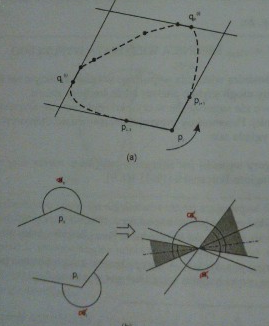
\includegraphics[width=0.3\textwidth]{img/diameter}
  \caption{Rysunek roboczy.\label{fig:diameter}}
\end{figure}

Wejściem dla algorytmu jest wielokąt zadany jako lista wierzchołków ze
wskaźnikiem na swój następnik w kolejności przeciwnej do ruchu
wskazówek zegara --- następnikiem wierzchołka $p_{n-1}$ jest
$p_0$. Dla czytelności algorytmu przyjmijmy także, że żadna para boków
tego wielokąta nie jest równoległa. Do określenia, który punkt leży
najdalej od odcinka $p_{i}p_{i+1}$, korzystamy z funkcji ,,podwojonego
pola ze znakiem trójkąta'' $p_{0}p_{i+1}p$, którą przedstawiono w
rozdziale~\ref{chap:pojecia} do wyznaczenia skrętności kąta. W
pierwszej części algorytmu w pętli \texttt{while} szukamy pierwszego
najdalszego wierzchołka i oznaczamy go jako $q_0$. Następnie
wyznaczamy łańcuch $C(p_i)$, używając wskaźników $p$ i $q$
poruszających się w kierunku odwrotnym do ruchu wskazówek zegara,
zaczynając odpowiednio od $p_0$ i $q_0$ do momentu, aż wskaźnik $q$
wróci do pozycji $p_0$. Po tym kroku zostaną wypisane wszystkie pary
antypodyczne. Znalezienie wierzchołka $q_0$ zajmuje w pesymistycznym
przypadku $N-1$ kroków, natomiast przejście po łańuchach $p_{0},
\ldots, q_{0}$ i $q_{0}, \ldots, p_{0}$ łącznie $N$ kroków. Mamy więc
do czynienia ze złożonością czasową rzędu $O(N)$.

% Specjalną sytuacją jest przypadek, gdy dwie krawędzie są równoległe
% (wtedy pole ze znakiem trójkąta jest równe dla dwóch wierzchołków
% tworzących krawędź równoległą), która wymaga od nas dodatkowego kroku
% przy każdym wierzchołku (wiersze 15--19).

% Poprawność algorytmu wynika z tego, że krawędzi równoległych jest co
% najwyżej $N/2$, więc łącznie algorytm nie wykonuje więcej niż $3N$
% kroków. Mamy więc do czynienia ze złożonością czasową rzędu $O(n)$.

Fakt, że punkt antypodyczny dla punktu $p_{i+1}$ nie może być bliższy
niż wierzchołek, który jest najdalej od $p_i$, wynika z wypukłością
wielokąta --- dla dowolnego wierzchołka $p$ można wyznaczyć taki
wierzchołek $q$, że odległość kolejnych wierzchołków od $p$ do $q$
jest nierosnąca, zaś od $q$ do $p$ --- niemalejąca.

\begin{figure}[htp]

  \begin{algorithmic}[1]
    \Procedure{Antipodal Pairs}{}

    \State $p \gets p_{n-1}$
    \State $q \gets NEXT[p]$

    \State

    \While {$NEXT[q]$ jest dalej od $(p, NEXT[p])$ niż $q$}
        \State {\emph{/* znajdźmy wierzchołek najdalszy od $(p, NEXT[p])$ */}}
        \State{$q \gets NEXT[p]$}

        \State

        \State {\emph{/* oznaczmy go jako $q_0$ */}}
        \State {$q_0 \gets q$}

        \State

        \While {$q \neq p_0$}
                \State {$p \gets NEXT[p]$}

                \State $print (p, q)$

                \State

                \While {$NEXT[q]$ jest dalej od odcinka $(p, NEXT[p])$ niż $q$}
                        \State $q \gets NEXT[q]$

                        \State

                        \State {\emph{/* jeżeli nie wróciliśmy do pozycji początkowej */ }}
                        \If {$(p, q) \neq (q_0,p_0)$}
                                \State $print (p, q)$
                        \EndIf
                \EndWhile
         \EndWhile
     \EndWhile
\EndProcedure

  \end{algorithmic}
  \caption{\label{alg:antipodal}}
\end{figure}

\begin{table}[htb]
  \centering

  \begin{tabular}{llll}
    \toprule
    $p$ & $q$ & para antypodyczna & krok \\
    \midrule
    $p_6$ & & & 1 \\
    \midrule
    & $p_0$ & & 3 \\
    \midrule
    & $p_1$ & & 5 \\
    \midrule
    & $p_2$ & & 5 \\
    \midrule
    & $p_3$ & & 5 \\
    \midrule
    $p_0$& & & 13 \\
    \midrule
    & & $(p_0, p_3)$ & 14 \\
    \midrule
    & $p_4$ & & 17 \\
    \midrule
    & & $(p_0, p_4)$ & 21 \\
    \midrule
    $p_1$& & & 13 \\
    \midrule
    & & $(p_1, p_4)$ & 14 \\
    \midrule
    & $p_5$ & & 17 \\
    \midrule
    & & $(p_1, p_5)$ & 21 \\
    \midrule
    $p_2$& & & 13 \\
    \midrule
    & & $(p_2, p_5)$ & 14 \\
    \midrule
    $p_3$& & & 13 \\
    \midrule
    & & $(p_3, p_5)$ & 14 \\
    \midrule
    & $p_6$ & & 17 \\
    \midrule
    & & $(p_3, p_6)$ & 21 \\
    \midrule
    & $p_0$ & & 17 \\
    \bottomrule
  \end{tabular}

  \caption{Ilustracja działania algorytmu  \textsc{Antipodal Pairs} dla
    wielokąta z rysunku~\ref{fig:antipodal}.}
\end{table}

%%% Local Variables:
%%% mode: latex
%%% TeX-master: "masterthesis"
%%% TeX-engine: xetex
%%% End:

\chapter{Przecięcie wielokątów}
Problem znalezienia przecięcia dla wielokątów wypukłych zdefiniowany
jest następująco.

\begin{problem}[Przecięcie wielokątów]
  Mając dane dwa wielokąty wypukłe $P$ i $Q$, znaleźć ich
  \emph{przecięcie} tj.\ obszar należący jednocześnie do $P$ i do $Q$.
\end{problem}

W niniejszym rozdziale do wielokąta będziemy zaliczać jego wnętrze
wraz z brzegiem. Jako $n$ będziemy oznaczać liczbę wierzchołków $P$, a
jako $m$ liczbę wierzchołków $Q$. Stosując algorytm naiwny polegający
na sprawdzeniu przecięcia każdej krawędzi $P$ z każdą krawędzią $Q$
można uzyskać punkty wszystkich przecięć w czasie $O(nm)$.

\section{Algorytm Shamosa-Hoeya}
Podstawową metodą rozwiązywania problemów w algorytmice jest technika
\emph{dziel i zwyciężaj}, które polega na podziale na mniejsze części,
znajdowaniu rozwiązań częściowych, a następnie łączeniu ich w końcowy
rezultat.

Metodę wykorzystującą podział płaszczyzny, dla problemu przecięcia
wielokątów zaproponowali Shamos i Hoey~\cite{ShamosHoey76}. Przez
każdy wierzchołek $P$ i $Q$ prowadzimy prostą pionową, tworząc w ten
sposób $n+m$ nieskończonych prostokątów zwanych dalej \emph{pasami}
(rysunek~\ref{img:ShamosHoey76}). Znalezienie przecięć krawędzi obydwu
wielokątów w każdej warstwie pozwoli nam na proste wyznaczenie obszaru
przecięcia tych wielokątów. Wynika to z poniższego twierdzenia.

\begin{twierdzenie}[Shamos-Hoey 1976]
  Przecięcie wielokątów wypukłych $P = (p_1, \ldots, p_n)$ i $Q =
  (q_1, \ldots, q_m)$ jest wielokątem wypukłym o sumie wierzchołków
  nie większej niż $n + m$.
\end{twierdzenie}

\begin{proof}
  Przecięcie $P$ i $Q$ jest przecięciem $n + m$ wewnętrznym
  półpłaszczyzn wyznaczonych przez krawędzie obydwu wielokątów.
\end{proof}

Zauważmy, że w każdym pasie proste go ograniczające wraz z krawędziami
wielokąta tworzą trójkąt lub czworobok
(rysunek~\ref{img:ShamosHoey76}). Natomiast w pojedynczym pasie
przecięcie dwóch czworoboków (trójkątów) możemy wyznaczyć w czasie
stałym.

\begin{figure}[htb]
  \centering
  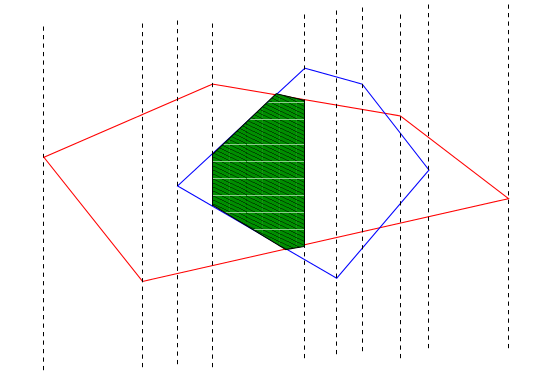
\includegraphics[scale=0.5]{img/ShamosHoey76}
  \caption{Podział na pasy a przecięcie
    wielokątów.\label{img:ShamosHoey76}}
\end{figure}

Następnie w czasie liniowym łączymy uzyskane kawałki i usuwamy
nadmiarowe wierzchołki powstałe przy podziale płaszczyzny. Początkowy
podział płaszczyzny również możemy przeprowadzić w czasie liniowym,
tak więc złożoność czasowa całego algorytmu wynosi $O(n + m)$.

\section{Algorytm O'Rourke-Chien-Olson-Naddor}
Kolejna metoda, zaproponowana przez O'Rourke i in.~\cite{Orourke98},
jest rozwinięciem algorytmu naiwnego.

Załóżmy, że $P$ i $Q$ przecinają się, oraz oznaczmy ich przecięcie $P
\cap Q$ jako $R$. Przyjmijmy również, że żadne dwie krawędzie z $P$ i
$Q$ nie są do siebie równoległe. Zauważmy, że brzeg $R$ składa się z
ciągu krawędzi należących do $P$, a następnie z ciągu krawędzie
należących do $Q$ (rysunek~\ref{img:sickles}). Jeżeli dany fragment
brzegu $R$ należy do $Q$, to jest on ,,objęty'' na zewnątrz przez ciąg
krawędzi $P$. I na odwrót --- fragmenty brzegu $R$, które należą do
$P$, są otoczone przez krawędzie należące do $Q$.

\begin{figure}[htb]
  \centering
  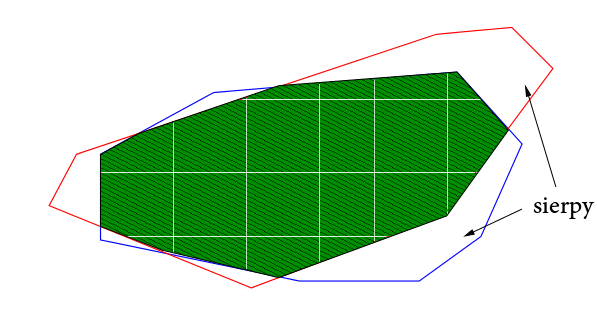
\includegraphics[scale=0.5]{img/Orourke98}
  \caption{Sierpy a przecięcie wielokątów.\label{img:sickles}}
\end{figure}

Możemy zauważyć, że przechodząc w odpowiedniej kolejności,
jednocześnie po zewnętrznych i wewnętrznych krawędziach ,,sierpa''
(rysunek~\ref{img:sickles}) ograniczymy sprawdzanie przecięć jedynie
do krawędzi początkowych i końcowych danego sierpa. Z tego względu
przy wyborze krawędzi, do której mamy przejść w danym kroku, kierujemy
się tym, czy krawędź bieżąca może zawierać przecięcie, które dopiero
ma być wykryte. Algorytm można przedstawić w postaci pseudokodu z
listingu~\ref{alg:Orourke98}.

\begin{figure}[htp]

  \begin{algorithmic}[1]
    \Procedure{Intersection of Convex Polygons}{}

    \State {$A \gets (p_0, p_1) \in P$}
    \State {$B \gets (q_0, q_1) \in Q$}

    \Repeat
    \State {sprawdź przecięcie krawędzi $A$ z krawędzią $B$}
    \State {w zależności od warunków przejdź po $A$ lub po $B$}
    \Until {$A$ i $B$ nie ,,okrążą'' swoich wielokątów}

    \EndProcedure
  \end{algorithmic}
  \caption{Algorytm wyznaczania przecięcia metodą O'Rourke i
    in.\label{alg:Orourke98}}
\end{figure}

Wybierzmy dowolną krawędź $A \in P$ oraz dowolną krawędź $B \in
Q$. Będziemy przechodzić po krawędziach obu wielokątów w kierunku
przeciwnym do ruch wskazówek zegara. W każdym kroku sprawdzamy
przecięcie bieżących krawędzi wielokątów $P$ i $Q$, i wybieramy
krawędź, do której podążymy w następnym kroku.  Chcemy kierować się
następującą regułą: jeżeli krawędź $B$ jest ,,skierowana'' w kierunku
krawędzi $A$, ale jej nie przecina, to zbliżamy się do $A$ przechodząc
po krawędzi $Q$ w miejsce możliwego przecięcia, w przeciwnym przypadku
przechodzimy po $B$.

\begin{figure}[htb]
  \centering
  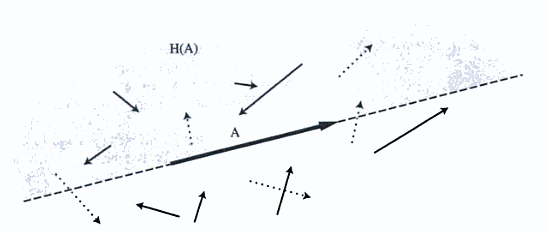
\includegraphics[scale=0.7]{img/vectors}
  \caption{\label{img:advance}}
\end{figure}

Rozważmy sytuację z rysunku~\ref{img:advance}. Niech $H(A)$ oznacza
półpłaszczyznę po lewej stronie skierowanej prostej współliniowej do
krawędzi $A$. Pogrubiona strzałka to wektor krawędzi $A$, pozostałe to
wektory krawędzi $B$.  Jako $A \times B > 0$ zapiszmy warunek, taki że
współrzędna $z$ iloczynu wektorowego wektorów krawędzi $A$ i $B$ jest
dodatnia (na rysunku~\ref{img:advance} oznaczone linią ciągłą). Jako
$a$ oznaczmy ,,skierowany'' wierzchołek należący do krawędzi $A$, zaś
jako $b$ ,,skierowany'' wierzchołek należący do krawędzi $B$. Przy
wyborze krawędzi, po której przejdziemy w bieżącym kroku stosujemy
poniższą regułę. Jeżeli

\begin{center}
  $A \times B > 0 $ i $b \notin H(A)$ lub $A \times B < 0 $ i $b \in
  H(A)$,
\end{center}

to przechodzimy po $B$. W przypadku przeciwnym przechodzimy po $A$.

Jeżeli $P$ i $Q$ przecinają się, to przecięcie zostanie znalezione po
$O(n+m)$ krokach. Znając punkty przecięć, dodatkowe $n+m$ kroków
wystarcza do wyznaczenia wszystkich wierzchołków tworzących brzeg
przecięcia $P \cap Q$. Możemy tym samym stwierdzić, że jeżeli po
$2(n+m)$ krokach nie odnajdziemy przecięcia to krawędzie $P$ i $Q$ nie
przecinają się. Na koniec, jeżeli nie odnotowano przecięcia krawędzi,
pozostaje sprawdzanie trzech końcowych warunków z
listingu~\ref{alg:OrourkeFinalTerms}. Sprawdzenie, czy punkt zawiera
się w wielokącie, tak jak to zostało pokazane w
rozdziale~\ref{chap:point_location}, dla wielokąta prostego można
wykonać w czasie liniowym, stąd złożoność czasowa całego algorytmy
wynosi $O(n + m)$.

\begin{figure}
  \begin{algorithmic}[1]
    \If {$p_i$ leży w $Q$}
    \State $P$ zawiera się $Q$
    \Else
    \If {$q_j$ leży w $P$}
    \State $Q$ zawiera się $P$
    \Else
    \State $P$ i $Q$ nie przecinają się
    \EndIf
    \EndIf
  \end{algorithmic}
  \caption{\label{alg:OrourkeFinalTerms}}
\end{figure}

\section{Algorytm Toussainta}
Stosunkowo prosty koncepcyjnie i implementacyjnie algorytm, działający
w czasie liniowym, zaproponował Toussaint w~\cite{ToussaintInt}.

\begin{figure}[htb]
  \centering
  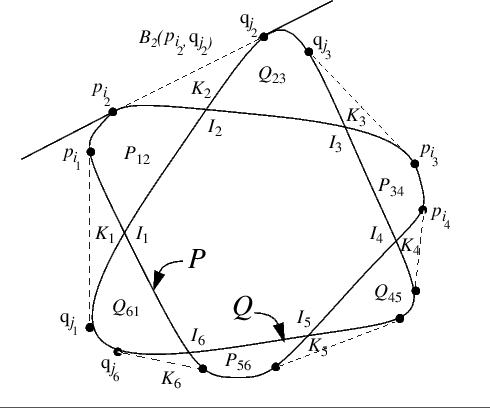
\includegraphics[scale=0.7]{img/toussaint1}
  \caption{\label{img:toussaint1}}
\end{figure}

\subsection{Opis}
Rozważmy dwa przecinające się wypukłe wielokąty $P$ i $Q$ oraz otoczkę
wypukłą sumy tych wielokątów $CH(P \cup Q)$
(rysunek~\ref{img:toussaint1}). Niech brzegi $P$ i $Q$ przecinają się
w $k$ punktach $I_1, I_2, \ldots, I_k$ ponumerowanych zgodnie z ruchem
wskazówek zegara. Brzegi $P$ i $Q$ oraz otoczka wypukła $CH(P \cup Q)$
dzielą płaszczyznę na $2k + 1$ ograniczonych regionów: obszar
przecięcia wielokątów $P \cap Q$ wyznaczony przez punkty $I_1, I_2,
\ldots, I_k$, $k$ regionów gdzie $P$ lub $Q$ należy do otoczki
wypukłej $CH(P \cup Q)$, ale nie należy do obszaru $P \cap Q$
przecięcia tych wielokątów, oraz analogiczne $k$ ,,kieszeni'' $K_1,
K_2, \ldots, K_k$ leżących wewnątrz otoczki wypukłej $CH(P \cup Q$),
ale leżących na zewnątrz $P \cup Q$. Każdej kieszeni $K_v$
przypisujemy odpowiadający jej punkt przecięcia $I_v$ oraz krawędź
otoczki $CH(P \cup Q)$, którą będziemy nazywać \emph{mostem}, łączącą
wierzchołek $p_i$ wielokąta $P$ oraz wierzchołek $q_j$ wielokąta $Q$ i
oznaczymy ją jako $B_{v}(p_{i_v}, q_{j_v})$. Cały algorytm
wyznaczający przecięcie wielokątów $P$ i $Q$ można przedstawić w
trzech krokach (listing~\ref{alg:interconpol}).

\begin{figure}[htp]
  \begin{algorithmic}[1]
    \Procedure{Alogrytm Interconpol}{}

    \State \emph{/* krok 1 */)}

    \State wyznacz otoczkę wypukłą $CH(P \cup Q)$

    \State

    \If {$CH(P \cup Q) = P$ (lub $Q$)}
    \State zwróć $Q$ (lub $P$) jako przecięcie

    \Else
    \State kontynuuj
    \EndIf

    \State

    \State \emph{/* krok 2 */}

    \State \textbf{dla każdego} mostu z $CH(P \cup Q)$:
    \State \hspace{\algorithmicindent} znajdź odpowiadający mu punkt
    przecięcia
    \State \textbf{end}

    \State

    \State \emph{/* krok 3 */}

    \State połącz wewnętrzne łańcuchy należące do $P$ i $Q$

    wyznaczone przez punkty przecięcia znalezione w poprzednim kroku

    \EndProcedure
  \end{algorithmic}
  \caption{\label{alg:interconpol}}
\end{figure}


\subsection{Poprawność}
Poprawność algorytmu opiera się na poniższych lematach.

\begin{lemat}
  Jeżeli $P$ i $Q$ przecinają się to dla każdego mostu $CH(P \cup Q)$
  istnieje jeden związany z nim punkt przecięcia $P \cap Q$.
\end{lemat}

\begin{proof}
  Oznaczmy jako $L(u, v)$ skierowaną prostą przechodzącą przez $u$ i
  $v$ w kierunku z $u$ do $v$, oraz oznaczmy jako $RH(u, v)$
  półpłaszczyznę na prawo od $L(u, v)$. Analogicznie, jako $LH(u, v)$
  oznaczmy półpłaszczyznę leżącą na lewo od $L(u, v)$.

  Niech $B(p_i, q_j)$ będzie mostem
  (rysunek~\ref{img:toussaint2}). $L(p_i, q_j)$ jest prostą
  wspierającą dla $P$ i $Q$ jednocześnie, więc $P$ i $Q$ muszą leżeć w
  półpłaszczyźnie $RH(p_i, q_j)$. Przejdźmy po brzegu $P$ zaczynając
  od $p_i$ w kierunku zgodnym z ruchem wskazówek zegara, dopóki nie
  natrafimy na krawędź wielokąta $P$ przecinającą krawędź wielokąta
  $Q$. Punkt przecięcia oznaczmy jako $I$. Analogicznie przejdźmy po
  brzegu $Q$ zaczynając od $q_j$ w kierunku przeciwnym do ruchu
  wskazówek zegara, dopóki nie natrafimy na krawędź wielokąta $Q$
  przecinającą krawędź wielokąta $P$. Z wypukłości obu wielokątów
  wynika, że tym razem punktem przecięcia również jest $I$ i w ten
  sposób jest on związany z mostem $B(p_i, q_j)$.

  Z drugiej strony załóżmy, że $I$ jest pewnym punktem przecięcia
  pomiędzy krawędziami $(p_k, p_{k+1}) \in P$ i $(q_l, q_{l+1}) \in
  Q$. Ponieważ $P \in RH(p_k, p_{k+1})$ oraz $Q \in RH(q_l, q_{l+1})$,
  to żadna krawędź inna niż $(p_k, p_{k+1})$ i $(q_l, q_{l+1})$ nie
  może przecinać się w regionie $R = RH(p_{k+1}, p_k) \cap RH(q_{l+1},
  q_l)$. Dodatkowo, ponieważ $\angle p_{k}Iq_{l+1} < 180^{\circ}$,
  musi istnieć krawędź $(p_i, q_j) \in CH(P \cup Q)$, która przecina
  region $R$ i jest nią most odpowiadający punktowi przecięcia $I$.
\end{proof}

\begin{figure}[htb]
  \centering
  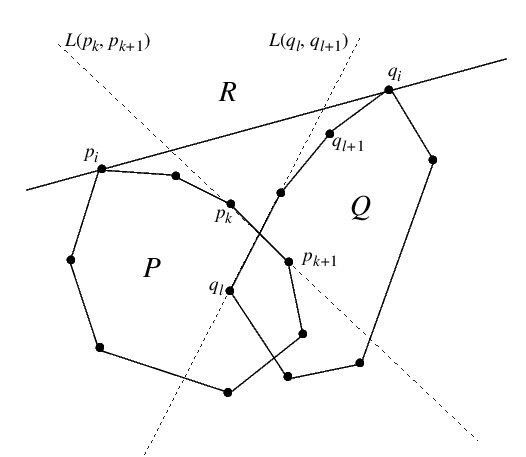
\includegraphics[scale=0.7]{img/toussaint2}
  \caption{\label{img:toussaint2}}
\end{figure}

\begin{twierdzenie}[Toussaint 1985\label{thm:toussaint85}]
  Algorytm poprawnie wyznacza punkt przecięcia dla odpowiadającego mu
  mostu.
\end{twierdzenie}

Zanim omówimy dowód powyższego twierdzenia wprowadźmy definicje.

\begin{definicja}
  Łańcuchem $C(p_i,p_{i+1},\ldots,p_j)$ będziemy nazywać ciąg
  kolejnych, następujących po sobie krawędzi i wierzchołków
  wielokąta prostego zaczynając od wierzchołka $p_i$ do wierzchołka
  $p_j$. Jeżeli każda krawędź łańcucha wraz z następną krawędzią
  tworzy kąt prawoskrętny to taki łańcuch nazywamy
  \emph{wypukłym}. Analogicznie, jeżeli każda krawędź wraz ze swoim
  następnikiem tworzy kąt lewoskrętny to taki łańcuch nazywamy
  \emph{łańcuchem wklęsłym}.
\end{definicja}

\begin{definicja}
  Wielokątem \emph{żaglokształtnym} będziemy nazywać wielokąt
  zawierający krawędź $(p_{i}p_{i+1})$ będącą \emph{masztem} oraz
  wierzchołek $p_j$, który będziemy \emph{czubkiem żagla}, połączony z
  wierzchołkami $p_i$ i $p_{i+1}$ \emph{łańcuchami wklęsłymi}.
\end{definicja}

\begin{definicja}
  Odcinek leżący w wielokącie $P$ i łączący dwa nie sąsiadujące
  wierzchołki wielokąta $P$ nazywamy \emph{przekątną} $P$.
\end{definicja}

\begin{definicja}\label{def:ear}
  Niech $p_i, p_{i+1}, p_{i+2}$ będą trzema kolejnymi, następującymi
  po sobie wierzchołkami należącymi do wielokąta $P$. Jeżeli przekątna
  łącząca $p_{i}$ i $p_{i+2}$ leży w $P$ to punkt $p_i$ nazywamy
  \emph{uchem} wielokąta $P$.
\end{definicja}

Zauważmy, że każda kieszeń wraz z odpowiadającym jej mostem oraz
punktem przecięcia $I_i$ tworzy wielokąt
\emph{żaglokształtny}. Ponadto mamy następujący lemat.

\begin{lemat}\label{lem:sailtip}
  Czubek wielokąta żaglokształtnego jest uchem.
\end{lemat}

\begin{figure}[htb]
  \centering
  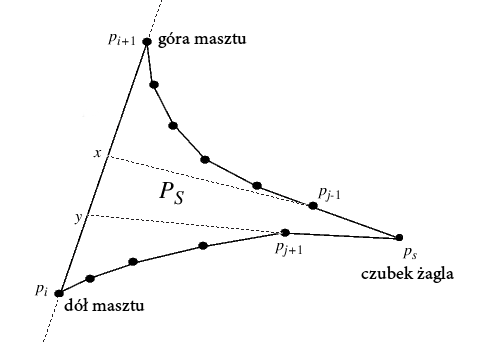
\includegraphics[scale=0.7]{img/toussaint3}
  \caption{\label{img:toussaint3}}
\end{figure}

\begin{proof}
  Przedłużmy krawędzie $(p_j,p_{j-1})$ i $(p_j, p_{j+1})$ tak, by
  przecinały linię $L(p_i, p_{i+1})$ odpowiednio w punktach $x$ i $y$
  (rysunek~\ref{img:toussaint3}). Ze względu na to, że $p_j$ jest
  połączony z $p_i$ łańcuchem wypukłym, punkt $x$ musi leżeć na
  odcinku $(p_i, p_{i+1})$ będącym masztem $P$. Analogicznie, punkt
  $y$ musi leżeć na maszcie $P$. Punkty $p_j, p_{j-1}, x, y, p_{j+1},
  p_j$, tworzą obszar znajdujący się w całości w $P$, stąd przekątna
  $(p_{j-1}, p_{j+1})$ również musi leżeć w $P$.
\end{proof}

\begin{twierdzenie}[Meisters 1975\label{thm:meisters}] Każdy wielokąt o
  $n$ krawędziach ($n > 3$) ma co najmniej dwoje nienachodzących na
  siebie uszu.
\end{twierdzenie}

\begin{lemat}\label{lem:sailmast}
  Uchem jest góra masztu wielokąta żaglokształtnego albo uchem jest
  jego dół.
\end{lemat}

\begin{proof}
  Z definicji~\ref{def:ear} wiemy, że tylko wierzchołki wypukłe mogą
  być uszami, a więc w wielokącie żaglokształtnym $P$ uszami mogą być
  jedynie $p_i$, $p_{i+1}$ oraz $p_j$. Z lematu~\ref{lem:sailtip}
  wiemy, że $p_j$ musi być uchem. Z twierdzenia~\ref{thm:meisters}
  wiemy, że $P$ musi mieć co najmniej dwoje uszu. Stąd albo $p_i$ albo
  $p_{i+1}$ musi być uchem.
\end{proof}

\begin{proof}[Dowód twierdzenia~\ref{thm:toussaint85}]
  W każdym zachowywany jest następujący niezmiennik: po obcięciu
  kolejnego ucha pozostała cześć wielokąta również jest wielokątem
  żaglokształtnym.

  Lemat~\ref{lem:sailtip} pozwala nam na triangulację $P$ w każdym
  kroku obcinając ucho będące górą lub dołem masztu, dopóki nie
  dojdziemy do czubka żagla i krawędzi z niego wychodzących.
\end{proof}

W naszym przypadku wierzchołek $p_j$ jest szukanym punktem przecięcia
$I_i$, tak więc dodatkowo w algorytmie powinniśmy uwzględnić warunek
sprawdzający czy w bierzącym kroku nadal rozważamy krawędź należącą do
wielokąta żaglokształtnego. Kompletny algorytm znajdujący czubek żagla
wielokąta $P$ został przedstawiony na listingu~\ref{alg:stepdown}.

\begin{figure}[htp]
  \begin{algorithmic}[1]
    \Procedure{Stepdown}{}

    \State $i \gets 1$
    \State $j \gets 1$

    % \State

    \Repeat
    \State $koniec \gets true$

    % \State

    \While{$\angle p_{i}p_{i+1}q_{j+1}$ jest lewoskrętny}
    \State $j \gets j + 1$
    \State $koniec \gets false$
    \EndWhile

    % \State

    \While{$\angle q_{j}q_{j+1}p_{i+1}$ jest prawoskrętny}
    \State $i \gets i + 1$
    \State $koniec \gets false$
    \EndWhile

    \Until{$koniec$}

    % \State

    \State $p_s \gets p_i$
    \State $q_t \gets q_j$

    \EndProcedure
  \end{algorithmic}
  \caption{\label{alg:stepdown}}
\end{figure}

Wejściem dla procedury jest most $B_k(p_i,p_j)$ należący do $CH(P \cup
Q)$, a wyjściem para wierzchołków $p_s$ i $q_t$, gdzie $(p_s,p_{s+1})
\cap (q_t,q_{t+1})$ wyznacza punkt przecięcia $I_k$. Warunki ,,$\angle
p_{i}p_{i+1}q_{j+1}$ jest lewoskrętny'' oraz ,,$\angle
q_{j}q_{j+1}p_{i+1}$ jest prawoskrętny'' w pętlach \textbf{while}
zapewniają, że w każdym kroku odetniemy ucho oraz że nie przejdziemy
przez czubek żagla. Przebieg działania procedury \textsc{Stepdown} dla
mostu z rysunku~\ref{fig:bridge} przedstawiają
rysunki~\ref{fig:stepdown1}--\ref{fig:stepdown5}.

\subsection{Złożoność}
Niech $n$ oznaczana liczbę wierzchołków wielokąta $P$, a $m$ liczbę
wierzchołków wielokąta $Q$. Znalezienie otoczki wypukłej dwóch
przecinających się wielokątów wypukłych może być wykonane w czasie
$O(m + n)$\cite{Toussaint83}. W~\cite{ToussaintInt}, Toussaint
proponuje wykorzystać technikę \emph{rotating calipers}, pozwalającą w
tym samym czasie stwierdzić, czy $CH(P \cup Q) = P$ lub $CH(P \cup Q)
= Q$.

Procedura znajdująca przecięcie $I_k$ jest wywoływana $k$ razy. Każde
wywołanie wymaga czasu liniowego zależnego od liczby wierzchołków
należących do danego żagla. Wszystkich takich wierzchołków może być
maksymalnie $n + m$, stąd ta część algorytmu wymaga czasu $O(n + m)$.

Ostatnią część algorytmu, połączenie uzyskanych łańcuchów wewnętrznych
można wykonać w czasie liniowym przechodząc przez krawędzie obydwu
wielokątów, jeżeli podczas szukania punktów przecięć oznaczyliśmy
kierunek w którym dana część wielokąta staje się łańcuchem
wewnętrznym.

Stąd złożoność czasowa całego algorytmu wynosi $O(n + m)$.

\begin{figure}[tp]
  \centering
  \begin{tikzpicture}
    \coordinate (q4) at (6, 5);
    \coordinate (q3) at (4, 4.5);
    \coordinate (q2) at (2.5, 3.5);
    \coordinate (q1) at (1.5, 1.5);
    \coordinate (q0) at (2, -0.25);
    \coordinate (q6) at (5, 0);
    \coordinate (q5) at (7, 2);

    \draw [blue] (q0) -- (q1) -- (q2) -- (q3) -- (q4) --  (q5) -- (q6) -- cycle;

    \node [anchor=center,circle,draw,fill,inner sep=1pt,
    label={250:$q_0$}] at (q0) {};

    \node [anchor=center,circle,draw,fill,inner sep=1pt,
    label={left:$q_1$}] at (q1) {};

    \node [anchor=center,circle,draw,fill,inner
    sep=1pt,label={right:$q_2$}] at (q2) {};

    \node [anchor=center,circle,draw,fill,inner
    sep=1pt,label={below:$q_3$}] at (q3) {};

    \node [anchor=center,circle,draw,fill,inner
    sep=1pt,label={above:$q_4$}] at (q4) {};

    \node [anchor=center,circle,draw,fill,inner
    sep=1pt,label={right:$q_5$}] at (q5) {};

    \node [anchor=center,circle,draw,fill,inner
    sep=1pt,label={below:$q_6$}] at (q6) {};

    \coordinate (p4) at (2, 3);
    \coordinate (p3) at (1, 4.5);
    \coordinate (p2) at (-1, 5);
    \coordinate (p1) at (-3, 3);
    \coordinate (p0) at (0, 0);
    \coordinate (p5) at (2, 1);

    \draw [red] (p0) -- (p1) -- (p2) -- (p3) --  (p4) -- (p5) -- cycle;

    \node [anchor=center,circle,draw,fill,inner sep=1pt,
    label={right:$p_1$}] at (p1) {};

    \node [anchor=center,circle,draw,fill,inner
    sep=1pt,label={above:$p_2$}] at (p2) {};

    \node [anchor=center,circle,draw,fill,inner
    sep=1pt,label={below:$p_3$}] at (p3) {};

    \node [anchor=center,circle,draw,fill,inner
    sep=1pt,label={left:$p_4$}] at (p4) {};

    \node [anchor=center,circle,draw,fill,inner
    sep=1pt,label={right:$p_5$}] at (p5) {};

    \node [anchor=center,circle,draw,fill,inner
    sep=1pt,label={below:$p_0$}] at (p0) {};

    \draw [dashed, shorten >= -2cm, shorten <= -2cm] (p2) -- (q4);
  \end{tikzpicture}
  \caption{Przerywaną linią oznaczono most.\label{fig:bridge}}
\end{figure}


\begin{figure}[htp]
  \centering
  \begin{tikzpicture}
    \coordinate (q4) at (6, 5);
    \coordinate (q3) at (4, 4.5);
    \coordinate (q2) at (2.5, 3.5);
    \coordinate (q1) at (1.5, 1.5);
    \coordinate (q0) at (2, -0.25);
    \coordinate (q6) at (5, 0);
    \coordinate (q5) at (7, 2);

    \draw [blue] (q1) -- (q2) -- (q3) -- (q4);

    \node [anchor=center,circle,draw,fill,inner sep=1pt,
    label={}] at (q1) {};

    \node [anchor=center,circle,draw,fill,inner
    sep=1pt,label={}] at (q2) {};

    \node [anchor=center,circle,draw,fill,inner
    sep=1pt,label={below:$q_{j+1}$}] at (q3) {};

    \node [anchor=center,circle,draw,fill,inner
    sep=1pt,label={above:$q_j$}] at (q4) {};

    \coordinate (p4) at (2, 3);
    \coordinate (p3) at (1, 4.5);
    \coordinate (p2) at (-1, 5);
    \coordinate (p1) at (-3, 3);
    \coordinate (p0) at (0, 0);
    \coordinate (p5) at (2, 1);

    \draw [red] (p2) -- (p3) --  (p4) -- (p5);

    \node [anchor=center,circle,draw,fill,inner
    sep=1pt,label={above:$p_i$}] at (p2) {};

    \node [anchor=center,circle,draw,fill,inner
    sep=1pt,label={left:$p_{i+1}$}] at (p3) {};

    \node [anchor=center,circle,draw,fill,inner
    sep=1pt,label={}] at (p4) {};

    \node [anchor=center,circle,draw,fill,inner
    sep=1pt,label={}] at (p5) {};

    \draw (p2) -- (q4);
    \draw [dashed] (p2) -- (q3);
  \end{tikzpicture}
  \caption{Kąt $\angle{p_{i}p_{i+1}q_{j+1}}$ jest lewoskrętny więc
    odcinamy ucho $q_j$.\label{fig:stepdown1}}
\end{figure}

\begin{figure}[htp]
  \centering
  \begin{tikzpicture}
    \coordinate (q4) at (6, 5);
    \coordinate (q3) at (4, 4.5);
    \coordinate (q2) at (2.5, 3.5);
    \coordinate (q1) at (1.5, 1.5);
    \coordinate (q0) at (2, -0.25);
    \coordinate (q6) at (5, 0);
    \coordinate (q5) at (7, 2);

    \draw [blue] (q1) -- (q2) -- (q3) -- (q4);

    \node [anchor=center,circle,draw,fill,inner sep=1pt,
    label={}] at (q1) {};

    \node [anchor=center,circle,draw,fill,inner
    sep=1pt,label={}] at (q2) {};

    \node [anchor=center,circle,draw,fill,inner
    sep=1pt,label={below:$q_{j}$}] at (q3) {};

    \node [anchor=center,circle,draw,fill,inner
    sep=1pt,label={right:$q_{j+1}$}] at (q2) {};

    \coordinate (p4) at (2, 3);
    \coordinate (p3) at (1, 4.5);
    \coordinate (p2) at (-1, 5);
    \coordinate (p1) at (-3, 3);
    \coordinate (p0) at (0, 0);
    \coordinate (p5) at (2, 1);

    \draw [red] (p2) -- (p3) --  (p4) -- (p5);

    \node [anchor=center,circle,draw,fill,inner
    sep=1pt,label={above:$p_i$}] at (p2) {};

    \node [anchor=center,circle,draw,fill,inner
    sep=1pt,label={left:$p_{i+1}$}] at (p3) {};

    \node [anchor=center,circle,draw,fill,inner
    sep=1pt,label={}] at (p4) {};

    \node [anchor=center,circle,draw,fill,inner
    sep=1pt,label={}] at (p5) {};

    \draw (p2) -- (q3);
    \draw [dashed] (q3) -- (p3);
  \end{tikzpicture}
  \caption{Kąt $\angle{p_{j}p_{j+1},q_{i+1}}$ jest prawoskrętny więc
    odcinamy ucho $p_i$.}
\end{figure}

\begin{figure}[htp]
  \centering
  \begin{tikzpicture}
    \coordinate (q4) at (6, 5);
    \coordinate (q3) at (4, 4.5);
    \coordinate (q2) at (2.5, 3.5);
    \coordinate (q1) at (1.5, 1.5);
    \coordinate (q0) at (2, -0.25);
    \coordinate (q6) at (5, 0);
    \coordinate (q5) at (7, 2);

    \draw [blue] (q1) -- (q2) -- (q3) -- (q4);

    \node [anchor=center,circle,draw,fill,inner sep=1pt,
    label={}] at (q1) {};

    \node [anchor=center,circle,draw,fill,inner
    sep=1pt,label={}] at (q2) {};

    \node [anchor=center,circle,draw,fill,inner
    sep=1pt,label={below:$q_{j}$}] at (q3) {};

    \node [anchor=center,circle,draw,fill,inner
    sep=1pt,label={right:$q_{j+1}$}] at (q2) {};

    \coordinate (p4) at (2, 3);
    \coordinate (p3) at (1, 4.5);
    \coordinate (p2) at (-1, 5);
    \coordinate (p1) at (-3, 3);
    \coordinate (p0) at (0, 0);
    \coordinate (p5) at (2, 1);

    \draw [red] (p2) -- (p3) --  (p4) -- (p5);

    \node [anchor=center,circle,draw,fill,inner
    sep=1pt,label={}] at (p2) {};

    \node [anchor=center,circle,draw,fill,inner
    sep=1pt,label={left:$p_{i}$}] at (p3) {};

    \node [anchor=center,circle,draw,fill,inner
    sep=1pt,label={left:$p_{i+1}$}] at (p4) {};

    \node [anchor=center,circle,draw,fill,inner
    sep=1pt,label={}] at (p5) {};

    \draw (q3) -- (p3);
    \draw [dashed] (p3) -- (q2);

  \end{tikzpicture}
  \caption{Kąt $\angle{p_{i}p_{i+1}q_{j+1}}$ jest lewoskrętny więc
    odcinamy ucho $q_j$.}
\end{figure}

\begin{figure}[htp]
  \centering
  \begin{tikzpicture}
    \coordinate (q4) at (6, 5);
    \coordinate (q3) at (4, 4.5);
    \coordinate (q2) at (2.5, 3.5);
    \coordinate (q1) at (1.5, 1.5);
    \coordinate (q0) at (2, -0.25);
    \coordinate (q6) at (5, 0);
    \coordinate (q5) at (7, 2);

    \draw [blue] (q1) -- (q2) -- (q3) -- (q4);

    \node [anchor=center,circle,draw,fill,inner sep=1pt,
    label={250:$q_{j+1}$}] at (q1) {};

    \node [anchor=center,circle,draw,fill,inner
    sep=1pt,label={}] at (q3) {};

    \node [anchor=center,circle,draw,fill,inner
    sep=1pt,label={right:$q_{j}$}] at (q2) {};

    \coordinate (p4) at (2, 3);
    \coordinate (p3) at (1, 4.5);
    \coordinate (p2) at (-1, 5);
    \coordinate (p1) at (-3, 3);
    \coordinate (p0) at (0, 0);
    \coordinate (p5) at (2, 1);

    \draw [red] (p2) -- (p3) --  (p4) -- (p5);

    \node [anchor=center,circle,draw,fill,inner
    sep=1pt,label={}] at (p2) {};

    \node [anchor=center,circle,draw,fill,inner
    sep=1pt,label={left:$p_{i}$}] at (p3) {};

    \node [anchor=center,circle,draw,fill,inner
    sep=1pt,label={left:$p_{i+1}$}] at (p4) {};

    \node [anchor=center,circle,draw,fill,inner
    sep=1pt,label={}] at (p5) {};

    \draw (p3) -- (q2);
    \draw [dashed] (p4) -- (q2);
  \end{tikzpicture}
  \caption{Kąt $\angle{q_{j}q_{j+1}p_{i+1}}$ jest prawoskrętny więc
    odcinamy ucho $p_i$.}
\end{figure}

\begin{figure}[htp]
  \centering
  \begin{tikzpicture}
    \coordinate (q4) at (6, 5);
    \coordinate (q3) at (4, 4.5);
    \coordinate (q2) at (2.5, 3.5);
    \coordinate (q1) at (1.5, 1.5);
    \coordinate (q0) at (2, -0.25);
    \coordinate (q6) at (5, 0);
    \coordinate (q5) at (7, 2);

    \draw [blue] (q1) -- (q2) -- (q3) -- (q4);

    \node [anchor=center,circle,draw,fill,inner sep=1pt,
    label={250:$q_{j+1}$}] at (q1) {};

    \node [anchor=center,circle,draw,fill,inner
    sep=1pt,label={}] at (q3) {};

    \node [anchor=center,circle,draw,fill,inner
    sep=1pt,label={right:$q_{j}$}] at (q2) {};

    \coordinate (p4) at (2, 3);
    \coordinate (p3) at (1, 4.5);
    \coordinate (p2) at (-1, 5);
    \coordinate (p1) at (-3, 3);
    \coordinate (p0) at (0, 0);
    \coordinate (p5) at (2, 1);

    \draw [red] (p2) -- (p3) --  (p4) -- (p5);

    \node [anchor=center,circle,draw,fill,inner
    sep=1pt,label={}] at (p2) {};

    \node [anchor=center,circle,draw,fill,inner
    sep=1pt,label={}] at (p3) {};

    \node [anchor=center,circle,draw,fill,inner
    sep=1pt,label={left:$p_{i}$}] at (p4) {};

    \node [anchor=center,circle,draw,fill,inner
    sep=1pt,label={right:$p_{i+1}$}] at (p5) {};

    \draw (p4) -- (q2);
  \end{tikzpicture}
  \caption{Kąt $\angle{p_{i}p_{i+1}q_{j+1}}$ jest prawoskrętny, a kąt
    $\angle{q_{j}q_{j+1}p_{i+1}}$ lewoskrętny, algorytm kończy
    działanie.\label{fig:stepdown5}}
\end{figure}

%%% Local Variables:
%%% mode: latex
%%% TeX-master: "masterthesis"
%%% TeX-engine: xetex
%%% End:

\chapter{Algorytmy z wykorzystaniem techniki \emph{rotating calipers}}
Użyty w rozdziale~\ref{chap:diameter} algorytm można zobrazować jako
zestaw obracających się suwmiarek i jako ogólną metodę można
zastosować przy rozwiązywaniu innych problemów geometrycznych dla
wielokątów wypukłych, pozwalająca na uzyskanie algorytmów działających
w czasie $O(n)$.

\section{Wyznaczanie średnicy}
W tej sekcji zostanie przedstawiony algorytm wyznaczania średnicy z
poprzedniego rozdziału w kontekście techniki \emph{rotating calipers}.

% \subsection{Opis algorytmu}
Niech $P = (p_1, p_2, \ldots, p_n)$ będzie wielokątem
wypukłym. Algorytm z rozdziału \ref{chap:diameter} znajduję wszystkie
pary antypodyczne, a następnie wybiera tę parę, która jest najbardziej
od siebie oddalona, będącą średnicą (na podstawie
tw. \ref{thm:yagbol}). Do znalezienia punktów antypodycznych możemy
użyć suwmiarki składającej się z dwóch równoległych linii
wsparcia. Rozważmy rysunek (). Jako początkową pozycję linii wsparcia
wyznaczmy prostą równoległą do osi $x$ przechodząca przez wierzchołek
$P$ położony najwyżej względem osi $y$ oraz równoległą do niej prostą
przechodząca przez wierzchołek $P$ położony najniżej na osi
$y$. Punkty $p_i$ i $p_j$ są pierwszą znalezioną parą
antypodyczną. Aby znaleźć następną, rozważmy kąty, które tworzy linia
wsparcia przechodząca przez $p_i$ z krawędzią $(p_i, p_{i+1})$ oraz
linia wsparcie przechodząca przez $p_j$ z krawędzią $(p_j, p_{j+1})$.
Jeżeli $\angle{\theta_j} < \angle{\theta_i}$ to obracamy linie
wsparcia o kąt $\theta_j$, w przeciwnym przypadku obracamy linie
wsparcia o kąt $\theta_i$. Punkty $(p_{j+1}, p_i)$ stają się następną
parą antypodyczną. Proces powtarzamy do momentu gdy linie wsparcia
wykonają pełny obrót tj. gdy $p_j = p_{i_0}$ i $p_i = p_{j_0}$.

% rysunek

% pseudokod

\section{Najmniejszy prostokąt zawierający}
Problem najmniejszego prostokąta zawierającego zdefiniujmy
następująco:

\begin{problem}[Najmniejszy prostokąt zawierający]
  Dla wielokąta wypukłego $P$ znaleźć najmniejszy prostokąt taki, żeby
  $P$ był w nim zawarty.
\end{problem}

Rozwiązanie tego problemu ma swoje zastosowanie m. in. w przetwarzaniu
obrazów, grach komputerowych i pewnych algorytmach dotyczących
optymalnego upakowania.

Algorytm z wykorzystaniem suwmiarek opiera się na twierdzeniu:

\begin{twierdzenie}[Freeman-Shapira]
  Najmniejszy prostokąt zawierający wielokąt $P$, posiada bok
  \emph{kolinearny} z bokiem $P$.
\end{twierdzenie}

Jako $L_s(p_i)$ będziemy oznaczać skierowaną linię wsparcia wielokąta
w wierzchołku $p_i$, taką, że $P$ znajduję się po prawej stronie
linii. Rozważmy rysunek (). W pierwszym kroku znajdujemy wierzchołki,
o minimalnych i maksymalnych współrzędnych $x$ i $y$. Oznaczmy te
wierzchołki jako $p_i$, $p_j$, $p_k$, $p_l$. Niech para linii
$L_s(p_j)$ i $L_s(p_l)$ będzie \emph{suwmiarką} pierwszą suwmiarką,
natomiast para $L_s(p_i)$, $L_s(p_k)$ drugą. Analogicznie jak w
algorytmie wyznaczającym średnice, mamy tym razem do rozważenia cztery
kąty: $\angle{\theta_i}, \angle{\theta_j}, \angle{\theta_k},
\angle{\theta_l}$. Obróćmy teraz wszystkie cztery linie wsparcia o
najmniejszy z nich. Wyznaczmy pole prostokąta wyznaczonego przez
punkty przecięć linii wsparcia $L_s(p_i), L_s(p_j), L_s(p_k)$ i
$L_s(p_l)$. Czynność tą powtarzamy z nowo powstałymi kątami
$\angle{\theta_i}, \angle{\theta_j}, \angle{\theta_k},
\angle{\theta_l}$ do czasu gdy rozpatrzone zostaną wszystkie możliwe
prostokąty zawierające tj. obydwie suwmiarki wykonają pełny obrót
wokół $P$. Ze wszystkich wyznaczonych w ten sposób prostokątów
zawierający wybieramy najmniejszy.

\section{Największa odległość\label{sec:max_dist}}
\begin{problem}
  Niech $P = (p_1, p_2, \ldots, p_n)$ oraz $Q = (q_1, q_2, \ldots,
  q_n)$ będą wielokątami wypukłymi. Największą odległość między $P$ i
  $Q$ oznaczamy jako $d_{\max}(P, Q)$ i definiujemy jako: $d_{\max}(P,
  Q) = \max{\{ d(p_i, q_j) \mid i, j = 1, 2, \ldots, n \}}$ gdzie
  $d(p_i, q_j)$ oznacza odległość euklidesową pomiędzy $p_i$ i $q_j$.
\end{problem}

Należy zauważyć, że największa odległość między dwoma wielokątami
wypukłymi nie musi być równa średnicy otoczki wypukłej $P \cup Q$,
więc nie możemy wykorzystać algorytmu wyznaczającego średnicę do
rozwiązania tego problemu.

Rozważmy rysunek (). W pierwszym kroku znajdźmy dwa punkty z których
jeden $p_i$ należy do $P$, a drugi $q_j$ do $Q$, tak aby linie
wsparcia $L_s(p_i)$ i $L_s(p_j)$ były równoległe. Możemy na przykład
wybrać punkty o skrajnym położeniu względem osi $y$. Niech $L_s(p_i)$
i $L_s(q_j)$ będą liniami skierowanymi w przeciwnych
kierunkach. Utworzone w ten sposób linie wsparcia tworzą kąt
$\angle{\theta_i}$ z krawędzią $(p_i, p_{i+1}) \in P$ oraz
kat$\angle{\phi_j}$ z krawędzią $(q_j, q_{j+1}) \in Q$. Wyznaczamy
odległość między $p_i$ i $q_j$. Wybieramy mniejszy z kątów $\phi$ i
$\theta$, a następnie obracamy obydwie linie wsparcia o ten
kąt. Proces powtarzamy do czasu gdy linie wsparcia wykonają pełny
obrót wokół wielokątów. W ostatnim kroku wybieramy najmniejszą z
wyznaczonych odległości między punktami.

\section{Łączenie otoczek wypukłych}
\begin{problem}
  Dla $CH(P)$ i $CH(Q)$ będącymi \emph{otoczkami wypukłymi} zbiorów $P$ i
  $Q$, znaleźć otoczkę wypukłą $CH(CH(P) \cup CH(Q))$.
\end{problem}

W algorytmach typu \emph{dziel i rządź} wyznaczających otoczkę wypukłą
zbioru punktów, końcowym etapem jest łączenie otoczek uzyskanych w
poprzednim kroku, uzyskując w ten sposób coraz większe otoczki, aż do
uzyskania otoczki wypukłej całego zbioru. Jeśli łącznie zostałoby
przeprowadzone w czasie liniowym, złożoność czasowa całego algorytmu
wyniesie $O(n \log n)$[].

Rozważmy dwa wielokąty wypukłe $P$ i $Q$ będącymi otoczkami wypukłymi
pewnych zbiorów punktów (rys). W tym przypadku wyznaczenie otoczki
wypukłej obydwu wielokątów wymaga znalezienia dwóch par wierzchołków
$p_i, p_j$ oraz $q_k, q_l$, takich, że krawędzie $(p_i, q_k)$ i $(p_j,
q_l)$, wraz z łańcuchami wypukłymi $(p_i, p_{i+1}, \ldots, p_j)$ i
$(q_k, q_{k+1}, \ldots, q_l)$ tworzy $CH(P \cup Q)$. Krawędzie $(p_i,
q_k)$ i $(p_j, q_l)$ będziemy nazywać \emph{mostami}, a wierzchołki
tworzące most będziemy nazywać \emph{punktami mostu}.

Algorytm wykorzystujący suwmiarki do wyznaczania mostów opiera się na
następującym twierdzeniu:

\begin{twierdzenie}
\label{thm:bridge}
  Dwa wierzchołki $p_i \in P$ i $q_j \in Q$ są \emph{punktami mostu}
  wtedy i tylko wtedy, gdy tworzą \emph{parę kopodalną} i wierzchołki
  $p_{i-1}, p_{i+1}, q_{j-1}, q_{j+1}$ leżą po tej samej stronie
  prostej $L(p_i, q_j)$.
\end{twierdzenie}

\begin{definicja}
  Para kopodalna
\end{definicja}

Po wyznaczeniu pozycji suwmiarek, analogicznie jak w algorytmie
\ref{sec:max_dist}, skierowanych w przeciwnych kierunkach, zaczynamy
obracać je wokół wielokątów. Podobnie jak w poprzednich problemach
rozważamy kąt jaki tworzy skierowana linia wsparcia wielokąta $P$ w
punkcie $p_i$ z krawędzią $(p_{i+1}, p_{i+2})$ oraz linia wsparcia
wielokąta $Q$ z krawędzią $(q_{j+1}, q_{j+2})$. Obydwie suwmiarki
obracamy o mniejszy z tych kątów. Przed każdym kolejnym obrotem
sprawdzamy czy aktualna para wierzchołków $p_i, q_j$ spełnia warunek
zawarty w tw.\ref{thm:bridge}. Ponieważ przy każdym obrocie suwmiarek
generowana jest nowa para kopodalną, pozostaje sprawdzić czy
wierzchołki $p_{i-1}, p_{i+1}, q_{j-1}, q_{j+1}$ leżą po tej samej
stronie prostej $L(p_i, q_j)$. Algorytm znajdowania mostów w przypadku
łączenia otoczek rozdzielnych wypukłych, tak jak ma to miejsce w
przypadku algorytmu dziel i rządź wyznaczania otoczki wypukłej zbioru
punktów, można zakończyć po znalezieniu obydwu mostów.

Niech liczba wierzchołków $P$ wynosi $n$, a liczba wierzchołków $Q$
wynosi $m$. Par ko-podalnych jest $k < n + m$. Sprawdzenie czy para
ko-podalna jest mostem odpobywa się w czasie $O(1)$, stąd złożoność
czasowa algorytmu wyznaczającego mosty jest liniowa i wynosi $O(k)$.

%%% Local Variables:
%%% mode: latex
%%% TeX-master: "masterthesis"
%%% TeX-engine: xetex
%%% End:

\chapter{Zawieranie wielokątów}
Ogólny problem zawierania wielokątów formułujemy następująco.

\begin{problem}
  Dla dwóch wielokątów prostych $P$ i $Q$ stwierdzić, czy $P$ może być
  zawarty w $Q$, i jeżeli tak, to podać \emph{umiejscowienie} $P$,
  które spełnia zawieranie.
\end{problem}

\begin{figure}[htb]
  \centering
  \begin{tikzpicture}
      \coordinate (p0) at (5.5,1.5);
      \coordinate (p1) at (3,4);
      \coordinate (p2) at (0,3);
      \coordinate (p3) at (-1,-0.5);
      \coordinate (p4) at (3,-2);

      \draw (p0) -- (p1) -- (p2) -- (p3) -- (p4) -- cycle;

      \node [anchor=center,circle,draw,fill,inner
      sep=1pt,label={right:$p_0$}] at (p0) {};

      \node [anchor=center,circle,draw,fill,inner
      sep=1pt,label={above:$p_1$}] at (p1) {};

      \node [anchor=center,circle,draw,fill,inner
      sep=1pt,label={left:$p_2$}] at (p2) {};

      \node [anchor=center,circle,draw,fill,inner
      sep=1pt,label={left:$p_3$}] at (p3) {};

      \node [anchor=center,circle,draw,fill,inner
      sep=1pt,label={below:$p_4$}] at (p4) {};

      \coordinate (q0) at (8,6);
      \coordinate (q1) at (4,7);
      \coordinate (q2) at (4,4);
      \coordinate (q3) at (6,4);

      \draw (q0) -- (q1) -- (q2) -- (q3) -- cycle;

      \node [anchor=center,circle,draw,fill,inner
      sep=1pt,label={right:$q_0$}] at (q0) {};

      \node [anchor=center,circle,draw,fill,inner
      sep=1pt,label={60:$q_1$}] at (q1) {};

      \node [anchor=center,circle,draw,fill,inner
      sep=1pt,label={left:$q_2$}] at (q2) {};

      \node [anchor=center,circle,draw,fill,inner
      sep=1pt,label={below:$q_3$}] at (q3) {};

      \coordinate (q0') at (4.5, 1.5);
      \coordinate (q1') at (0.5, 2.5);
      \coordinate (q2') at (0.5, -0.5);
      \coordinate (q3') at (2.5, -0.5);

      \draw [dashed] (q0') -- (q1') -- (q2') -- (q3') -- cycle;

      \node [anchor=center,circle,draw,fill,inner
      sep=1pt,label={right:$q_{0}'$}] at (q0') {};

      \node [anchor=center,circle,draw,fill,inner
      sep=1pt,label={60:$q_{1}'$}] at (q1') {};

      \node [anchor=center,circle,draw,fill,inner
      sep=1pt,label={left:$q_{2}'$}] at (q2') {};

      \node [anchor=center,circle,draw,fill,inner
      sep=1pt,label={below:$q_{3}'$}] at (q3') {};
  \end{tikzpicture}
  \caption{Wielokąt $(q_0, \ldots, q_3)$ można umieścić w wielokącie
    $(p_0, \ldots, p_4)$\label{img:containment1}}
\end{figure}

W problemie ogólnym dopuszczamy translacje i obroty zawieranego
wielokąta tak, by ,,zmieścił się'' on wielokącie
zawierającym. Rozwiązanie tego problemu w czasie $O(pq^2)$ w
przypadku, gdy $Q$ jest wielokątem wypukłym przedstawił Chazelle
w~\cite{Chazelle83}. Dla dowolnych wielokątów rozwiązanie naiwne
wymaga czasu $O[p^3q^3(p + q) \log{(p + q)}]$~\cite{Chazelle83}. W tej
samej pracy przedstawiono także rozwiązanie dla uproszczonego
problemu, w którym wielokąty $P$ i $Q$ są wypukłe, a dozwolonym
działaniem na $P$ jest jedynie translacja.

Niech będzie dany wielokąt wypukły $P = (p_0, p_2, \ldots, p_{n-1})$
oraz wielokąt wypukły $Q = (q_0, q_1, \ldots, q_{m-1})$. Dla
uproszczenia zakładamy, że żadna para krawędzi wielokątów $P$ i $Q$
nie jest do siebie równoległa. Niech $H_i$ dla $i = 0, \ldots, m - 1$
będzie $i$-tą półpłaszczyzną określoną przez prostą współliniową do
krawędzi $(q_i, q_{i+1})$ i zawierającą wielokąt $Q$. Niech punkt $c$
będzie dowolnym punktem należącym do $P$, może być to na przykład
środek jego masy. Punkt ten będzie wyznaczał umiejscowienie $P$ na
płaszczyźnie.

Gdy przesuniemy $P$ tak, by punkt $c$ znajdował się w jak najmniejszej
odległości od $H_i$, to jeden wierzchołek $p_j \in P$ będzie styczny z
prostą $L(q_i, q_{i+1})$ wyznaczającą półpłaszczyznę $H_i$. O takim
wierzchołku $p_j$ mówimy, że jest \emph{krytyczny} dla krawędzi $(q_i,
q_{i+1})$. Odległość punktu $c$ od półpłaszczyzny $H_i$ oznaczmy jako
$d_i$.

Rozważmy półpłaszczyznę $H_i'$ wyznaczoną przez prostą
$L'(q_i,q_{i+1})$ równoległą do $L(q_i, q_{i+1})$ i przechodzącą przez
punkt $c$. $L'(q_i,q_{i+1})$ możemy łatwo wyznaczyć, jeśli znamy
wierzchołek krytyczny dla $(q_i, q_{q+1})$. Zauważmy, że $P$ jest
zawarty w $Q$ wtedy i tylko wtedy, gdy jest zawarty w przecięciu
półpłaszczyzn $H_0 \cap \ldots \cap H_{m-1}$. Warunek ten jest
równoważny zawieraniu punktu $c$ w przecięciu półpłaszczyzn
$H_i'$. Innymi słowy: wielokąt $P$ zawiera się w $Q$ dokładnie wtedy,
gdy punkt $c$ należy do przecięcia półpłaszczyzn $H_i'$. Co więcej,
wspomniane przecięcie zawiera wszystkie możliwe umiejscowienia $c$
spełniające zawieranie $P$ w $Q$. Algorytm rozwiązujący problemu
zawierania wielokąta $P$ w $Q$ możemy przedstawić następująco.

\begin{figure}[htp]
\begin{algorithmic}[1]
\Procedure{Convex Polygon Containment}{}

\State \textbf{dla każdej} krawędzi $(q_i, q_{i+1}) \in Q$
\State \hspace{\algorithmicindent} wyznacz wierzchołek krytyczny $p_j \in P$
\State \hspace{\algorithmicindent} wyznacz półpłaszczyznę $H_i'$
\State \textbf{end}
\State wyznacz przecięcie otrzymanych półpłaszczyzn $H_i$

\EndProcedure
\end{algorithmic}
\end{figure}

Do znalezienia wierzchołków krytycznych możemy się posłużyć
przedstawioną w rozdziale \ref{chap:calipers} metodą \emph{rotating
  calipers}. Zauważmy, że dana krawędź $(q_i, q_{i+1})$ wraz z
odpowiadającym jej wierzchołkiem krytycznym $p_j$ tworzą parę
kopodalną. Niech początkowymi prostymi wspierającymi dla $P$ i $Q$
będą równoległe proste poziome, styczne do wierzchołka o najmniejszej
wartości współrzędnej $x$ z $P$ i $Q$ odpowiednio. Niech obydwie
proste wspierające będą skierowane w tym samym kierunku w ten sposób,
żeby wspierany wielokąt znajdował się po lewej stronie prostej
(rysunek~\ref{img:containment3}). Analogicznie jak w
rozdziale~\ref{chap:calipers} zaczynamy obracać równoległe proste
wspierające. Przy każdym obrocie suwmiarek, po którym prosta
wspierająca $L_{SQ}$ jest styczna z krawędzią $Q$, prosta wspierająca
$L_{SP}$ jest styczna z punktem krytycznym dla tej krawędzi. Następnie
dla każdej krawędzi $Q$ i odpowiadającemu jej punktowi krytycznemu
wyznaczamy półpłaszczyznę $H_i'$, tak jak zostało to opisane
wcześniej.

\begin{figure}[tb]
  \centering
  \begin{tikzpicture}
      \coordinate (p0) at (5.5,1.5);
      \coordinate (p1) at (3,4);
      \coordinate (p2) at (0,3);
      \coordinate (p3) at (-1,-0.5);
      \coordinate (p4) at (3,-2);

      \draw (p0) -- (p1) -- (p2) -- (p3) -- (p4) -- cycle;

      \node [anchor=center,circle,draw,fill,inner
      sep=1pt,label={right:$p_0$}] at (p0) {};

      \node [anchor=center,circle,draw,fill,inner
      sep=1pt,label={above:$p_1$}] at (p1) {};

      \node [anchor=center,circle,draw,fill,inner
      sep=1pt,label={left:$p_2$}] at (p2) {};

      \node [anchor=center,circle,draw,fill,inner
      sep=1pt,label={left:$p_3$}] at (p3) {};

      \node [anchor=center,circle,draw,fill,inner
      sep=1pt,label={below:$p_4$}] at (p4) {};

      \coordinate (q0) at (11,2);
      \coordinate (q1) at (7,3);
      \coordinate (q2) at (7,0);
      \coordinate (q3) at (9,0);

      \draw (q0) -- (q1) -- (q2) -- (q3) -- cycle;

      \node [anchor=center,circle,draw,fill,inner
      sep=1pt,label={right:$q_0$}] at (q0) {};

      \node [anchor=center,circle,draw,fill,inner
      sep=1pt,label={60:$q_1$}] at (q1) {};

      \node [anchor=center,circle,draw,fill,inner
      sep=1pt,label={left:$q_2$}] at (q2) {};

      \node [anchor=center,circle,draw,fill,inner
      sep=1pt,label={below:$q_3$}] at (q3) {};

      \draw [blue, <-, shorten <= -2cm, shorten >= -2cm] (p2) -- (p1);

      \draw[blue, ->, shorten <= -4cm] (q1) -- +($(p2)-(p1)$);
  \end{tikzpicture}
  \caption{Pary punktów $(p_1,q_1)$ oraz $(p_2, q_1)$ to pary
    kopodalne.}
\end{figure}

Na koniec pozostaje wyznaczenie przecięcia półpłaszczyzn $H_1' \cap
\ldots \cap H_m'$. Uzyskane półpłaszczyzny podzielmy dwa zbiory: dolny
i górny. Niech w dolnym zbiorze znajdą się półpłaszczyzny wyznaczone
przez ,,dolną'' część wielokąta $Q$. Zacznijmy rozpatrywać kolejne
półpłaszczyzny z dolnego zbioru pod względem nierosnącego
współczynnika kierunkowego prostej $l_i$ określającej półpłaszczyznę
$H_i'$. Włóżmy dwie pierwsze proste na stos. Będziemy oznaczać
ostatnią prostą na stosie jako $l_o$, a przedostatnią jako $l_p$. Po
rozpatrzeniu każdej kolejnej półpłaszczyzny będziemy zachowywać
następujący niezmiennik: na stosie znajdują się te proste z ciągu
$l_1, \ldots, l_i$, które stanowią brzeg zbioru $H_1' \cap \ldots \cap
H_i'$. Postępujemy zgodnie z regułą, że jeżeli przecięcie obecnie
rozważanej prostej $l_i$ z ostatnia prostą na stosie $l_o$ leży na
lewo od przecięcia $l_o$ z przedostatnią prostą $l_p$ ze stosu, to
zdejmujemy $l_o$ ze stosu i wkładamy na stos prostą $l_i$. Tę metodę
obrazuje sytuacja z rysunku~\ref{img:containment2}. Na stos zostały
włożone proste $l, l_p, l_o$, rozważana jest prosta $l_i$. Punkt $q' =
l_i \cap l_o$ leży na lewo od $q = l_o \cap l_p$. Wobec tego
zdejmujemy nadmiarową prostą $l_o$ ze stosu, a wkładamy na niego
prostą $l_i$. Analogicznie postępujemy z zbiorem ,,górnych''
półpłaszczyzn. W ostatnim kroku łączymy uzyskane dwa obszary wypukłe,
poprzez wyznaczenie przecięcia par skrajnych półpłaszczyzn z
,,dolnej'' i ,,górnej'' otoczki.

\vspace{3cm}

\begin{figure}[ht]
  \centering
  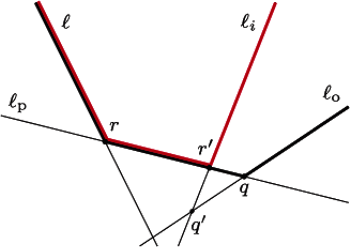
\includegraphics[scale=0.6]{img/containment2}
  \caption{\label{img:containment2} Czerwoną linią zaznaczono brzeg
    przecięcia półpłaszczyzn.}
\end{figure}

\cleardoublepage{}

\section{Poprawność}
Poprawność warunku zawierania $P$ w $Q$ jako warunku zawierania $P$ w
przecięciu półpłaszczyzn wyznaczonych przez krawędzie $Q$ opiera się
na następującym lemacie.

\begin{lemat}\emph{\cite{Chazelle83}}
  Przecięcie $n$ półpłaszczyzn jest obszarem wypukłym.
\end{lemat}

Lemat ten wynika bezpośrednio z poniższych własności.

\begin{itemize}
  \item Półpłaszczyzna jest zbiorem wypukłym.
  \item Przecięcie zbiorów wypukłych jest zbiorem wypukłym.
\end{itemize}

Drugim lematem, na którym opiera się algorytm jest:

\begin{lemat}\emph{\cite{Chazelle83}}
  Dla każdej krawędzi $Q$ istnieje wierzchołek krytyczny z $P$.
\end{lemat}

Zakładając, że żadne trzy wierzchołki $P$ nie są współliniowe, to z
wypukłości $P$ wynika, że istnieją co najwyżej dwa najbardziej
zbliżone do krawędzi $(q_i,q_{i+1})$ wierzchołki. Ma to miejsce w
przypadku, gdy krawędź $(q_i,q_{i+1})$ jest równoległa do krawędzi $P$
zawierającej obydwa wierzchołki krytyczne. W przeciwnym przypadku
istnieje dokładniej jeden wierzchołek krytyczny.

\begin{lemat}\emph{\cite{Chazelle83}}
  Algorytm poprawnie wyznacza dolne przecięcie półpłaszczyzn.
\end{lemat}

Rozważmy rysunek~\ref{img:containment2}, na którym przedstawiono zbiór
,,dolnych'' półpłaszczyzn. Możemy zauważyć, że półpłaszczyzna zadana
przez prostą $l_o$ jest nadmiarowa przy wyznaczeniu przecięcia $l \cap
l_p \cap l_o \cap l_i$. Jeżeli wyeliminujemy półpłaszczyzny
nadmiarowe, możemy w prosty sposób wyznaczyć przecięcie.

Dzięki temu, że nachylenie kolejnych półpłaszczyzn jest monotoniczne
(w przypadku ,,dolnego'' zbioru --- nierosnące), wystarczy, że
wyznaczymy punkty przecięć kolejnych pod tym względem półpłaszczyzn,
uzyskując w ten sposób zbiór punktów będących wierzchołkami obszaru
przecięcia. Do określenia, czy dana półpłaszczyzna jest nadmiarowa,
opieramy się na następującym założeniu.

\begin{lemat}\emph{\cite{Brown78}}
  Niech będą dane półpłaszczyzny $H_1, H_2, H_3$. Niech $l_i$ oznacza
  prostą kierunkową półpłaszczyzny $H_i$, natomiast jako $slope(l_i)$
  oznaczmy współczynniki kierunkowy prostej $l_i$. Półpłaszczyzna
  $H_2$ jest nadmiarowa dla określenia ,,dolnego'' przecięcia $H_1
  \cap H_2 \cap H_3$ dokładnie wtedy, gdy oba poniższe warunki są
  spełnione:

  \begin{enumerate}
    \item Prosta $l_2$ leży poniżej punktu przecięcia prostych $l_1$ i
      $l_3$.
    \item $slope(l_1) < slope(l_2) < slope(l_3)$.
  \end{enumerate}
\end{lemat}

Zauważmy, że warunek drugi jest spełniony ze względu na wypukłość
wielokąta. Natomiast do sprawdzenia warunku pierwszego wystarczające
jest sprawdzenie, czy przecięcie obecnie rozważanej prostej z ostatnią
prostą na stosie leży na lewo od przecięcia przedostatniej i ostatniej
prostej ze stosu. Gdy proste są uporządkowane według współczynnika
nachylenia, powyższe warunki są równoważne --- jeżeli $l_2$ przecina
$l_1$ na lewo od przecięcia $l_1$ i $l_3$, przecięcie $l_1 \cap l_2$
musi znajdować się powyżej prostej $l_3$.

\section{Złożoność}
Pierwszą część algorytmu, czyli wyznaczenie wierzchołków krytycznych,
dzięki zastosowaniu techniki \emph{rotating calipers} można wykonać w
czasie liniowym. Wyznaczenie początkowej pozycji prostych równoległych
wymaga rozpatrzenia wszystkich kolejnych wierzchołków wielokątów $P$ i
$Q$, stąd wymagany wynosi $O(n + m)$. Po każdym obrocie prostych
równoległych jedna z nich jest styczna do krawędzi wspieranego
wielokąta. Za każdym razem, gdy prosta równoległa jest styczna do
krawędzi wielokąta $Q$, wyznaczany jest punkt krytyczny dla tej
krawędzi. Tak więc po wykonaniu pełnego obrotu wokół $P$ i $Q$
wyznaczymy wszystkie wierzchołki krytyczne. Przechylenie prostej
równoległej do krawędzi wielokąta wykonujemy w czasie $O(1)$, stąd
pełny obrót obydwu prostych równoległych wokół wspieranych wielokątów
wymaga czasu $O(n + m)$.  Łącznie złożoność czasowa tej części
algorytmu również wynosi $O(n + m)$.

Odległość punktu $c$, wyznaczającego umiejscowienie $P$ na
płaszczyźnie, od krawędzi wielokąta $Q$ możemy wyznaczyć w czasie
$O(1)$, jeżeli wyznaczyliśmy wierzchołek krytyczny dla tej krawędzi.

W~\cite{Brown78} Brown dowodzi równoważności między problemem
przecięcia dolnych półpłaszczyzn, a problemem otoczki wypukłej, który
może być rozwiązany w czasie liniowo-logarytmicznym (lub w czasie
liniowym, jeżeli punkty otoczki są posortowane według kolejności
krążenia wokół środka układu współrzędnych). Rozważając złożoność tej
części algorytmu możemy również spojrzeć na rozwiązanie w następujący
sposób: wyznaczając górne oraz dolne przecięcie rozważamy kolejne
proste wkładając lub zdejmując je ze stosu. Każda prosta może być
włożona oraz zdjęta ze stosu tylko raz, stąd pozbycie się nadmiarowych
półpłaszczyzn z obu zbiorów przecięć wymaga czasu $O(n + m)$. Takiej
samej złożoności czasowej wymaga wyznaczenie dolnego oraz górnego
przecięcia z uzyskanych półpłaszczyzn oraz połączenie uzyskanych
obszarów wypukłych.

Stąd złożoność czasowa całego algorytmu wynosi $O(n + m)$.

%%% Local Variables:
%%% mode: latex
%%% TeX-master: "masterthesis"
%%% TeX-engine: xetex
%%% End:


\summary

\appendix
\chapter{Generowanie wielokątów wypukłych o zadanej liczbie
  wierzchołków}

\bibliographystyle{unsrt}
\bibliography{xml}

\listoftables
\listoffigures

\oswiadczenie

\end{document}

%%% Local Variables:
%%% coding: utf-8
%%% mode: latex
%%% TeX-master: t
%%% TeX-engine: xetex
%%% End:
